% NICOLE CAMILLE BAIÃO - PRAXISTRANSFERBERICHT III

% === DOKUMENTKLASSE ===
\documentclass[
    12pt, 
    a4paper,
    ]{scrartcl} % KOMA-Script-Artikelklasse mit deutscher Typografie

% === SPRACHE & ZEICHENSATZ ===
\usepackage[ngerman]{babel} % Deutsche Sprache und Silbentrennung
\usepackage{csquotes} % Typografisch korrekte Anführungszeichen

% === SEITENLAYOUT & FORMATIERUNG ===
\usepackage[a4paper, margin=2.5cm]{geometry}
\usepackage{setspace}
\setstretch{1.15}
\usepackage{fancyhdr}
\usepackage{float} % Exakte Platzierung von Gleitobjekten (z. B. Bilder)
\usepackage{caption} % Bild-/Tabellenbeschriftungen anpassen
\usepackage{adjustbox} % Elemente (z. B. Tabellen) skalieren oder ausrichten
\usepackage{makecell} % Mehrzeilige Zellen in Tabellen (Tabellen in Tabellen)
\usepackage{ragged2e}
\justifying 
% === SCHRIFTARTEN ===
\usepackage{iftex} % Prüft, ob XeTeX oder LuaTeX verwendet wird
\usepackage{fontspec} % Benutzerdefinierte Schriftarten (nur mit XeLaTeX/LuaLaTeX)
\usepackage{titlesec}
% Aktuelle Größen beibehalten:
\titleformat{\section}{\normalfont\fontsize{14}{5}\bfseries}{\thesection}{1em}{}
\titleformat{\subsection}{\normalfont\fontsize{13}{5}\bfseries}{\thesubsection}{1em}{}
\titleformat{\subsubsection}{\normalfont\fontsize{12}{5}\bfseries}{\thesubsubsection}{1em}{} 

% ABSTÄNDE ANPASSEN — Das ist der Schlüssel:
\titlespacing*{\section}{0pt}{1.1\baselineskip}{0.1\baselineskip}
\titlespacing*{\subsection}{0pt}{1.0\baselineskip}{0.1\baselineskip}
\titlespacing*{\subsubsection}{0pt}{0.9\baselineskip}{0.1\baselineskip}
 % Hauptschriftart
\setmainfont{Times New Roman} % Setzt Times New Roman als Hauptschrift

% === GRAFIKEN & ABBILDUNGEN ===
\usepackage{graphicx} % Bilder einfügen
\usepackage{xcolor} % Farben verwenden (z. B. in Code oder Text)
\usepackage{longtable}
\usepackage{tablefootnote}
% === QUELLEN & VERWEISE ===
\usepackage[
    colorlinks,       % Links ohne Umrandungen in gewählter Farbe
    linkcolor=black,  % Farbe interner Verweise
    filecolor=black,  % Farbe externer Verweise
    citecolor=black,  % Farbe von Zitaten
    urlcolor=black,    % Farbe von Links
    breaklinks
]{hyperref} % Verlinkungen
\usepackage{cleveref} % Querverweise der Querverweise
\newcommand{\etalchar}[1]{#1}

% === TABELLEN ===
\usepackage{longtable} % Tabellen über mehrere Seiten
% makecell wurde oben bereits geladen

% === CODE-DARSTELLUNG ===
\usepackage{listings} % Quellcode einfügen und formatieren

%%%%%%%%%%%%%%%%%%%%%%%%%%

% === ÜBERSCHRIFTEN-FORMATIERUNG ===
\setkomafont{sectioning}{\rmfamily\bfseries} % Überschriften fett und serifenlos

% === VERLINKUNGEN & REFERENZEN ===
\hypersetup{breaklinks=true} % Erlaubt Zeilenumbruch bei langen Links (wichtig für URLs oder Literaturverweise)
\newcommand{\anhang}[1]{\hyperref[#1]{\nameref{#1}}} % Eigener Befehl für Anhang-Verweise mit automatisch lesbarem Namen (anstatt z. B. nur "Abschnitt 5.1")

% === SEITENLAYOUT & RÄNDER ===
\geometry{
    verbose,
    tmargin=3cm,  % Oberer Rand
    bmargin=2cm,  % Unterer Rand
    lmargin=2.1cm,  % Linker Rand
    rmargin=3cm   % Rechter Rand
}

% === TYPOGRAFISCHE FEINHEITEN ===
\displaywidowpenalty = 5000
\widowpenalty=5000
\clubpenalty=5000
% === FUßNOTEN UND VERWEISE ===
\newcommand{\footfigref}[1]{\footnote{Abb. \ref{#1} auf Seite \pageref{#1}}} % Eigener Fußnotenbefehl für Bildverweise mit Seitenzahl

% === ABSTÄNDE & ABSATZFORMATIERUNG ===
\setlength{\footskip}{10mm} % Abstand zwischen Text und Fußzeile
\setlength{\abovecaptionskip}{4pt}  % Abstand oberhalb von Bild-/Tabellenunterschriften
\setlength{\belowcaptionskip}{0pt}  % Abstand unterhalb von Bild-/Tabellenunterschriften
\setlength{\intextsep}{1pc}         % Abstand bei Gleitobjekten (z. B. Bilder im Textfluss)
\setlength{\parindent}{0pt} % Kein Einzug am Absatzanfang
\setlength{\parskip}{0.75\baselineskip} % Einheitlicher Abstand zwischen Absätzen
\setstretch{1.5} % 1½-zeiliger Zeilenabstand
% === BILD- UND TABELLENUNTERSCHRIFTEN VERKLEINERN ===
\addtokomafont{caption}{\small} % Macht Bild-/Tabellenunterschriften kleiner

% === INHALTSVERZEICHNIS & LISTEN ===
\KOMAoptions{listof=entryprefix, toc=indent} % Inhaltsverzeichnis: eingerückt und mit Präfix bei Abbildungs-/Tabellenlisten

% === CODEDARSTELLUNG (SQL) ===
\lstdefinelanguage{SQL}{
    keywords={SELECT, FROM, WHERE, INSERT, INTO, VALUES, UPDATE, SET, DELETE, JOIN, LEFT, RIGHT, INNER, ORDER, BY, GROUP, ASC, DESC, CREATE, TABLE, PRIMARY, KEY, FOREIGN, ALTER, DROP, DATABASE, BEGIN, TRANSACTION, IF, EXISTS, COMMIT, AND},
    keywordstyle=\color{blue},           % Keywords blau
    comment=[l]{--},                     % Kommentare mit --
    morecomment=[s]{/*}{*/},             % Blockkommentare
    commentstyle=\color{gray},          % Kommentare grau
    stringstyle=\color{red},            % Strings rot
}

\lstset{
    basicstyle=\ttfamily\linespread{0.85}\selectfont,   % Standard-Monospace-Schrift für Listings
    keywordstyle=\bfseries\color{blue},  % Beispiel-Stil für Keywords
    commentstyle=\itshape\color{gray},   % Stil für Kommentare
    stringstyle=\color{red},            % Stil für Strings
    columns=flexible,       % Flexibler Zeilenumbruch
    language=SQL,
    breaklines=true
}

%%%%%%%%%%%%%%%%%%%%%%%%%%

% === BEGINN DOKUMENT ===
\begin{document}
% === LITERATUR EINBINDEN (alle Einträge aus der .bib ins Literaturverzeichnis) ===
\nocite{*}

% --- Seitenzahlen-Formatierung 1/3: Römische Zahlen ---
\pagenumbering{Roman}  % Nutzt römische Zahlen (I, II, III, …)
\pagestyle{fancy}      % Aktiviert fancyhdr für benutzerdefinierte Kopf-/Fußzeilen
\fancyhf{}             % Setzt alle Kopf- und Fußzeilen zurück
\fancyhead[R]{\thepage}  % Seitenzahl oben rechts anzeigen
\renewcommand{\headrulewidth}{0pt} % Keine Linie in der Kopfzeile
\renewcommand{\footrulewidth}{0pt} % Keine Linie in der Fußzeile

%%%%%%%%%%%%%%%%%%%%%%%%%%

% === BEGINN TITELSEITE ===
\begin{titlepage}
\begingroup
\setstretch{1.15} % Nur auf der Titelseite engerer Zeilenabstand
\centering % Zentriert den gesamten Inhalt der Titelseite
   
% --- Logos einfügen (links und rechts) ---

\includegraphics[scale=0.15]{BILDER-PTB3/Berliner-wasserbetriebe.svg.png}\hfill % \hfill sorgt dafür, dass die beiden Logos links und rechts stehen

\includegraphics[scale=0.25]{BILDER-PTB3/Hochschule_für_Wirtschaft_und_Recht_Berlin_logo.jpg} \\[0.5cm] % \\[1.8cm] fügt einen vertikalen Abstand von 1.8 cm nach den Bildern ein

% --- Titel (fette und große Schrift) ---
\Large{\textbf{Handlungsempfehlungen zur Optimierung von Schulungs- und Kommunikationsprozessen für zukünftige Microsoft 365-Anwendungen - basierend auf Microsoft Planner und To Do bei den Berliner Wasserbetriebe}} \\[0.4cm]

% --- Untertitel ---
{\Large Praxistransferbericht 3} \\

% --- Neuer Text mit Abstand --
\vspace{0.5cm} % Abstand zum Unterschift
\large % Setzt die Schriftgröße auf Standard
vorgelegt am 02.03.2026 an der\\ [0.2cm]
Hochschule für Wirtschaft und Recht Berlin\\ [0.2cm]
Fachbereich Duales Studium\\ [0.4cm]
\vspace{0.4cm} % Abstand zur Tabelle

% --- Tabelle mit persönlichen Angaben ---
{\large
\begin{tabular}{l l}  
    \textbf{von:} & Nicole Camille Baião  \\[0.1cm]
    \textbf{Bereich:} & Wirtschaft \\[0.1cm]
    \textbf{Fachrichtung:} & Wirtschaftsinformatik \\[0.1cm]
    \textbf{Studienjahrgang:} & 2024 \\[0.1cm]
    \textbf{Studienhalbjahr:} & 3. Semester \\[0.1cm]
    \textbf{Ausbildungsbetrieb:} & Berliner Wasserbetriebe  \\[0.1cm]
    \textbf{Betreuender Prüfer:} & Prof. Dr. Gert Faustmann \\[0.1cm]
    \textbf{Betreuer im Betrieb:} & Diana Ireri Jimenez Ireta \\[0.7cm]
\end{tabular}
}

% --- Bereich für Unterschriften ---
\raggedright % Setzt den folgenden Text linksbündig
\textbf{\normalsize{Von der Ausbildungsleiterin zur Kenntnis genommen:}} \\[0.8cm]

% --- Tabelle mit Unterschriften ---
\begin{tabular}{p{8cm} p{8cm}}
    \normalsize{Berlin, den 27. Februar 2026} & \normalsize{Berlin, den 27. Februar 2026} \\[0.03cm]

    
\includegraphics[width=5.7cm]{BILDER-PTB3/unterschrift_nicole.png} &
    \raisebox{-0.25cm}{
\includegraphics[width=3.3cm]{BILDER-PTB3/unterschrift_diana.png}} \\[-0.25cm]

    \normalsize{\underline{\hspace{5.5cm}}} & \normalsize{\underline{\hspace{5.5cm}}} \\[0.1cm]
    \normalsize{(Unterschrift der Studentin)} & \normalsize{(Unterschrift der Ausbildungsleiterin)}
\end{tabular}
% === ENDE TITELSEITE ===
\endgroup
\end{titlepage}

% === Inhaltsverzeichnis === 
\setcounter{page}{1} % Setzt die Seitennummer auf 1 für neue Zählung (Neustart der Zählung)
\newpage
\section*{Inhaltsverzeichnis}  
\renewcommand{\contentsname}{}
\vspace{-1.3cm}  % Anpassung des vertikalen Abstands
\tableofcontents % Inhaltsverzeichnis erstellen

% === Abküzungsverzeichnis === 
\newpage
\section*{Abkürzungsverzeichnis}  
\addcontentsline{toc}{section}{Abkürzungsverzeichnis}
\vspace{0.6cm}
\begin{tabular}{p{4cm} p{11.35cm}}   
    \textbf{\normalsize ADKAR:} & \normalsize Awareness, Desire, Knowledge, Ability, Reinforcement \\[0.5cm]
    \hline
    \textbf{\normalsize BPM:} & \normalsize Busnisses Process Management \\[0.5cm]
    \hline
    \textbf{\normalsize BWB:} & \normalsize Berliner Wasserbetriebe \\[0.5cm]
    \hline
    \textbf{\normalsize GPM:} & \normalsize Geschäftsprozessmanagement \\[0.5cm]
    \hline    
    \textbf{\normalsize IT-Z/M:} & \normalsize IT-Zentrale Aufgaben - Methoden und Werkzeuge \\[0.5cm]
    \hline
    \textbf{\normalsize IT-Z/R:} & \normalsize IT-Zentrale Aufgaben – Risk Compliance and Security \\[0.5cm]
 \end{tabular}

% --- Seitenzahlen-Formatierung 2/3: Wechsel auf normale (arabische) Zahlen ---
\newpage
\pagenumbering{arabic} % Normale Zahlen ab "Einleitung"
\setcounter{page}{1}
% === Einleitung ===
\section{Einleitung}
Die Berliner Wasserbetriebe (BWB) sind das größte Wasser- und Abwasserversorgungsunternehmen Deutschlands und zählen zu den größten Arbeitsgeber in Berlin. Mit rund 4.800\footnote{Vgl. \cite{BWB_Arbeitgeber}.} Mitarbeitenden und zahlreichen Fachabteilungen agiert das Unternehmen in einem komplexen organisatorischen Umfeld mit hohen regulatorischen Anforderungen, in dem IT-Abteilungen eine zentrale Rolle bei der Unterstützung und Weiterentwicklung digitaler Arbeitsprozesse einnimmt.

Die Digitalisierung der Arbeitswelt hat in den letzten Jahren erheblich an Bedeutung gewonnen. In vielen Unternehmen werden in diesem Zusammenhang neue digitale Anwendungen eingesetzt, um Arbeitsprozesse effizienter zu gestalten sowie die Zusammenarbeit und Kommunikation nachhaltig zu unterstützen. Ein Beispiel ist der Einsatz von Microsoft-365-Anwendungen in organisationalen Arbeitsumgebungen, wobei bei den BWB bereits Microsoft Planner und Microsoft To Do eingeführt wurden. Die Anwendungen sind technisch verfügbar und stehen den Mitarbeitenden grundsätzlich zur Nutzung bereit. In der Praxis zeigt sich jedoch, dass ihre Nutzung uneinheitlich erfolgt. Ein Teil der Mitarbeitenden ist nicht oder nur unzureichend über Existenz, Verfügbarkeit und Einsatzzweck der Anwendungen informiert, während andere Unsicherheiten bezüglich Funktionsumfang und sinnvoller Nutzung im Arbeitsalltag haben.

Die Planung, Steuerung und Begleitung der Anwendungen erfolgt bei der BWB innerhalb der IT-Z/M (Zentrale Aufgaben - Methoden und Werkzeuge). Dort werden standardisierte Schulungs- und Kommunikationsprozesse zur Einführung, Information und Nutzung der Anwendungen entwickelt, mit dem Ziel, eine einheitliche und nachvollziehbare Nutzung der bereitgestellten Tools im Unternehmen sicherzustellen. Die bestehenden Prozesse weisen jedoch Optimierungspotenziale auf, insbesondere im Hinblick auf Reichweite, Verständlichkeit und Nachhaltigkeit.

Ziel dieser Arbeit ist die Analyse der bestehenden Schulungs- und Kommunikationsprozesse im Zusammenhang mit Microsoft Planner und Microsoft To Do bei der BWB. Auf Grundlage einer qualitativen Analyse und Bewertung der IST-Prozesse nach den Prinzipien des Geschäftsprozessmanagements werden konzeptionelle SOLL-Prozesse abgeleitet, die als Orientierung für die zukünftige Gestaltung von Schulungs- und Kommunikationsprozessen im Microsoft-365-Umfeld dienen. Diese Ausarbeitung erfolgt in LaTeX.

\section{Theoretischer Rahmen}
\subsection{Grundlagen des Geschäftsprozessmanagement}
Die Begriffe \enquote{Geschäftsprozess} und \enquote{Prozess} werden in der Fachliteratur unterschiedlich definiert. Ein Prozess ist allgemein eine geordnete Abfolge von Tätigkeiten, die logisch zusammenhängen und ein bestimmtes Ziel verfolgen. Ein Geschäftsprozess ist ein spezieller Prozess, der zur Bearbeitung eines betriebswirtschaftlich relevanten Objekts durchgeführt wird. Er erhält Inputs von Lieferanten, verarbeitet das Objekt und liefert das Ergebnis als Output an seine Kunden.\footnote{Vgl. \cite{Koch_Geschaeftsprozessmanagement}, S.~2.} Das Geschäftsprozessmanagement (GPM) enthält keine einheitliche Definition und als synonym werden auch Begriffe wie Busnisses Process Management (BPM) oder Prozessmanagement verwendet. Gründsätzlich umfasst GPM die Planung, Steurung, Überwachung und Weiterentwicklung, den Prozessentwurft, die Prozessimplementierung sowie das Prozesscontrolling von Geschäftsprozessen in einer Organisation.\footnote{Vgl. \cite{Koch_Geschaeftsprozessmanagement}, S.~10.}

Das Geschäftsprozessmanagement basiert auf dem Zusammenwirken unterschiedlicher Rollen, die auf verschiedene Ebenen der Organisation angesiedelt sind und sowohl das operative Tagesgeschäft als auch die Weiterentwicklung von Geschäftsprozessen unterstützen. Der Chief Process Officer (CPO) trägt die Gesamtverantwortung für die Prozesse einer Organisation und ist für die Dokumentation, Restrukturierung und das Monitoring der Geschäftsprozesse zuständig. Zur bereichsübergreifenden Abstimmung und Steuerung von Prozessen wird häufig ein Process Steering Board bzw. Process Control Board eingerichtet, das übergreifende Prozessfragen klärt und Maßnahmen priorisiert.\footnote{Vgl. \cite{Gadatsch_Geschaeftsprozessmanagement}, S.~54-55.} Der Process Owner ist für die strategische und operative Steuerung eines Geschäftsprozesses verantwortlich und überwacht die Erreichung der definierten Prozessziele. Prozessmitarbeiter übernehmen überwiegend operative Aufgaben in den Prozessen und unterstützen durch ihre Fachkenntnisse die Umsetzung und kontinuierliche Verbesserung der Geschäftsprozesse. Definierten Rollen und Verantwortlichkeiten tragen dazu bei, Aufgaben im Rahmen des Geschäftsprozessmanagement klar zuzuordnen und Prozesse effizient zu steuern. Die strategische orientierte Gestaltung der Geschäftsprozesse erfolgt dabei im Kontext einer übergeordneten Prozessmanagement-Funktion, die die Ausrichtung und Koordination des GPM sicherstellt. 

Nach Gadatsch umfasst das Geschäftsprozessmanagement mehrere Aufgabenbereiche, die entlang des BPM-Lebenszyklus angesiedelt sind.\footnote{Vgl. \cite{Gadatsch_Geschaeftsprozessmanagement}, S.~56-57.} Diese beginnen mit der Projektvorbereitung, in der relevante Prozesse identifiziert, abgegrenzt, dokumentiert und modelliert werden. Darauf aufbauend erfolgt die Prozessanalyse mit dem Ziel, bestehende Schwachstellen zu erkennen. In der Phase der Prozessgestaltung bzw. -optimierung werden Prozesse neu gestaltet oder verbessert und entsprechende Prozessziele festgelegt. Anschließend schließtgschritt werden die definierten Prozesse organisatorisch und technisch umgesetzt, insbesondere durch die Implementierung in IT-Systeme wie Workflow-Management-Systeme. Die Prozessausführung und -überwachung dient der operativen Durchführung der Prozesse sowie der Kontrolle der Zielerreichung. Über alle Phasen hinweg stellt die übergreifende Prozesssteuerung die Koordination und Steuerung der Prozesse im gesamten BPM-Lebenszyklus sicher.\footnote{Vgl. \cite{Gadatsch_Geschaeftsprozessmanagement}, S.~55.}

\subsection{Prozessmodellierung und -bewertung}
Prozessmodelle werden als vereinfachte Abbildungen realer Prozesse innerhalb eines Unternehmens oder zwischen Unternehmen verstanden. Sie stellen die chronologisch-sachlogische Abfolge von Tätigkeiten dar und reduzieren die Komplexität realer Abläufe auf das für den jeweiligen Zweck notwendige Maß. Abhängig von der Zielsetzung unterscheiden sich Prozessmodelle hinsichtlich ihres Detaillierungsgrades und ihres Umfangs. Ziel der Prozessmodellierung ist es, Transparenz über Abläufe, Zuständigkeiten und Zusammenhänge zu schaffen, sodass alle Prozessbeteiligten ihre Aufgaben innerhalb der Prozesskette nachvollziehen können. Prozessmodelle unterstützen damit das Verständnis über Tätigkeiten, Funktionen, Rollen und Schnittstellen und tragen zur Erhöhung der Transparenz von Abläufen innerhalb und außerhalb der Organisation bei der Analyse.\footnote{Vgl. \cite{Koch_Geschaeftsprozessmanagement}, S.~47.}

Im Kontext von Schulungs- und Kommunikationsprozessen als unterstützende Geschäftsprozesse dient die Prozessmodellierung der strukturierten Darstellung von Abläufen, Informationsflüssen und Verantwortlichkeiten. Die Modellierung erfolgt auf Basis standardisierter Symbole und Notationen, um eine einheitliche Verständlichkeit sicherzustellen.\footnote{Vgl. \cite{Koch_Geschaeftsprozessmanagement}, S.~51.} Die verwendeten Symbole werden im Anhang erläutert.\footnote{Vgl. \hyperref[sec:Anhang1]{Anhang 1}.} 

\subsubsection{IST- und SOLL-Prozessen}
Die Modellierung von IST-Prozessen bildet die Grundlage für die Analyse bestehender Abläufe. Durch die strukturierte Erfassung der aktuellen Prozesssituation können Schwachstellen identifiziert und Verbesserungspotenziale herausgearbeitet werden. Eine hinreichende Kenntnis des Istzustandes ist Voraussetzung für die Entwicklung eines definierten Sollzustandes und für die Ableitung einer Migrationsstrategie vom Ist- zum Sollprozess. Darüber hinaus fördert die Istmodellierung bei den beteiligten Mitarbeitenden das Verständnis für fachliche Zusammenhänge und schafft eine gemeinsame Basis für die spätere Sollkonzeption.\footnote{Vgl. \cite{Koch_Geschaeftsprozessmanagement}, S.~65.} 

Die Soll-Modellierung baut auf den Erkenntnissen der Ist-Analyse auf und dient der gezielten Verbesserung von Strukturen und Abläufen. Ein Istmodell kann dabei als Leitfaden für das Sollkonzept genutzt werden, um sicherzustellen, dass keine relevanten Sachverhalte unberücksichtigt bleiben. Gleichzeitig ist zu beachten, dass die Erstellung von Istmodellen mit zeitlichem und organisatorischem Aufwand verbunden ist und nicht automatisch zu Prozessverbesserungen führt.\footnote{Ebenda, S.~65.}

\subsubsection{Qualitativen Bewertungskriterien}
Qualitative Bewertungsverfahren kommen dann zum Einsatz, wenn neben quantitativen auch qualitative Aspekte in die Bewertung von Lösungsalternativen einbezogen werden sollen oder wenn rein quantitative Wirtschaftlichkeitsbetrachtungen keine eindeutigen Ergebnisse liefern beziehungsweise nicht sinnvoll durchführbar sind. Sie dienen insbesondere dazu, nicht-monetäre Kriterien wie Qualität, Sicherheit oder inhaltliche Eignung systematisch zu berücksichtigen und auf dieser Grundlage eine Entscheidung für eine geeignete Lösung zu unterstützen.
Zu den qualitativen Bewertungsverfahren zählen unter anderem die Nutzwertanalyse, bei der Lösungsalternativen anhand zuvor festgelegter qualitativer Kriterien bewertet und in eine Rangfolge gebracht werden. Diese Kriterien bilden unterschiedliche qualitative Aspekte ab und drücken aus, in welchem Maß eine Alternative die angestrebten Ziele erfüllt.\footnote{Vgl. \cite{Koch_Geschaeftsprozessmanagement}, S.~97-98.} 
Die Prioritätenanalyse dient dazu, mehrere Kriterien oder Ziele nach ihrer relativen Bedeutung zu gewichten, um deren Einfluss auf eine Entscheidung transparent zu machen.\footnote{Vgl. \cite{Koch_Geschaeftsprozessmanagement}, S.~99-100.} Ergänzend ermöglicht die SWOT-Analyse eine qualitative Beurteilung, indem interne Stärken und Schwächen sowie externe Chancen und Risiken systematisch gegenübergestellt werden. Alle genannten Verfahren unterstützen die strukturierte Bewertung komplexer Sachverhalte auf Basis qualitativer Kriterien und werden im weiteren Verlauf der Arbeit gesondert erläutert.\footnote{Vgl. \cite{Koch_Geschaeftsprozessmanagement}, S.~100-101.}

\subsection{Veränderungsbegleitung mit ADKAR-Modell}
Das ADKAR-Modell ist ein Framework zur Analyse und Steuerung von Veränderungsprozessen auf individueller Ebene. Es basiert auf der Annahme, dass organisatorischer Wandel nur dann erfolgreich ist, wenn jede betroffene Person den Veränderungsprozess durchläuft. Ziel des Modells ist es, individuelles Verhalten systematisch zu beeinflussen und damit nachhaltige Veränderungen innerhalb von Organisationen zu ermöglichen.\footnote{Vgl. \cite{Prosci_ADKAR}, S.~4.}
Das Modell beschreibt fünf aufeinander aufbauende Zustände, die für eine erfolgreiche Veränderung erreicht werden müssen: Awareness (Bewusstsein für die Notwendigkeit der Veränderung), Desire (Bereitschaft zur Unterstützung der Veränderung), Knowledge (Wissen über die Umsetzung), Ability (Fähigkeit zur praktischen Anwendung) und Reinforcement (Sicherung und Verstetigung der Veränderung). Diese Elemente sind sequenziell und kumulativ zu verstehen, da jeder Schritt auf dem vorherigen aufbaut und Voraussetzung für eine nachhaltige individuelle Veränderung ist.\footnote{Vgl. \cite{Prosci_ADKAR}, S.~5.} Die dargestellte Methode wird in dem Anhang 3 anschaulich ergänzt.

  % === TEIL 2 ===
\section{Praxisanalyse: Planner und To Do bei den BWB}
% --- TEIL 2.1 ---
\subsection{Prozessverständnis von Einführung bis Kommunikation und Schulung}
Bei den BWB werden neue Software-Tools aus dem Microsoft-365-Paket schrittweise über ein formelles Beteiligungsverfahren eingeführt. Die Leiterin von Microsoft-365-Apps, Diana Jimenez, arbeitet im IT-Z/M und ist verantwortlich für die Schulungs- und Kommunikationsprozesse zur Einführung rund um diese Anwendungen. Sie beschreibt, dass sie bereits ab dem Moment einbezogen wird, „sobald ein Bedarf für eine neue Anwendung festgestellt wird“. In dieser Phase führt sie Tests durch, ob und wie die Anwendung für den Betrieb sinnvoll ist. Wenn das der Fall ist, dann beginnt sie mit der Erstellung von Vorlagen zu Schulungs- und Kommunikationsmaterialien – diese sind zunächst noch nicht-offizielle Entwürfe. Diese Vorlagen – etwa Präsentationen, Handbücher oder Tutorials – bereitet sie vor und stellt sie der Abteilung IT-Z/R (IT-Zentral Aufgaben - Risk, Compliance and Security) zur Verfügung. Erst nach der offiziellen Freigabe durch die Mitbestimmung finalisiert sie die endgültigen Schulungsunterlagen zur Veröffentlichung.\footnote{Vgl. \hyperref[sec:Anhang5]{Anhang 5}, Frage 1.}

Nicolas Zoll, Risikomanager aus IT-Z/R, beschreibt diesen Prozess als sehr aufwendig: Es müssen umfangreiche Dokumente erstellt werden, u. a. ein Whitepaper zur Beteiligung, eine fachliche Beschreibung der Anwendung, ein detailliertes Berechtigungskonzept, eine Schutzbedarfsfeststellung gemeinsam mit der Unternehmenssicherheit sowie datenschutzrechtliche Unterlagen wie ein Verzeichnis von Verarbeitungstätigkeiten (VVT), Löschkonzept und ggf. eine Datenschutz-Folgenabschätzung. Hinzu kommen Stellungnahmen des Datenschutzbeauftragten sowie der Datenschutzabteilung. All diese Dokumente werden in einer internen Vorabstimmung geprüft – oft unter Einbindung der Personalmanagement-Abteilung, also dem Gremium (PM-G) zur Freigabe vorgelegt. Erst wenn dieses Gremium zustimmt, wird der Antrag an den IT-Leiter und die Vorstandsrepräsentantin weitergeleitet und anschließend an den zuständigen Personalrat weitergeleitet, der die formale Mitbestimmung übernimmt.\footnote{Vgl. \hyperref[sec:Anhang6]{Anhang 6}, Frage 2.}

Dieser schulungsbezogene Teil ist eng in den umfassenderen Einführungsprozess eingebettet.\footnote{Vgl. \hyperref[sec:Anhang4]{Anhang 4}.} Die ganze Mitbestimmung ist Bestandteil des Prozesses, nimmt in der Regel viel Zeit in Anspruch und verzögert die Schulungs- und Kommunikationsprozesse. Erst wenn die Mitbestimmung abgeschlossen ist, darf die Anwendung offiziell produktiv eingeführt werden – und erst dann können Schulungs- und Kommunikationsmaßnahmen weitergeführt werden: Die Informationen über die neue Anwendung werden über das Intranetportal AQUA.net veröffentlicht. Zusätzlich werden Multiplikator:innen (ausgewählte Mitarbeitende) geschult, die das Wissen an weitere Mitarbeitende weitergeben. Ergänzend werden Online-Termine über Microsoft Teams angeboten sowie ergänzende Formate wie E-Mail-Ankündigungen, Workshops und Anwendungsbetreuung organisiert. Ziel ist es, durch abgestimmte Kommunikation und Schulungsangebote möglichst viele Mitarbeitende zu informieren und zur aktiven Anwendung zu befähigen.\footnote{Vgl. \hyperref[sec:Anhang 5]{Anhang 5}, Frage 1.} Die Arbeit enthält ein internes BWB-Dokument zum Beteiligungsprozess.\footnote{Vgl. \hyperref[sec:Anhang2]{Anhang 2}.}
% --- TEIL 2.2 ---
\subsection{SWOT-Analyse der Schulungsprozesse}
Die Schulungsmaßnahmen zur Einführung von Microsoft Planner und To Do bei den BWB bestehen aus einer Kombination von Selbstlernmaterialien (Tutorials, Handbücher, Präsentationen, Videos) sowie Online-Schulungen und Live-Workshops, ergänzt durch ein Multiplikatoren-Modell.\footnote{Vgl. \hyperref[sec:Anhang5]{Anhang 5}, Frage 2.} Trotz dieses breiten Angebots zeigt sich in der Praxis eine uneinheitliche Nutzung der Tools.\footnote{Vgl. \hyperref[sec:Anhang5]{Anhang 5}, Frage 4.} Die folgende SWOT-Analyse beleuchtet die Stärken, Schwächen, Chancen und Risiken der aktuellen Schulungsprozesse:
\begin{itemize}
    \setlength\itemsep{0.4\baselineskip}
    \setlength\parskip{0pt}
    \setlength\parsep{0pt}
    \item \textbf{Stärken (Strengths):} Die vorhandenen Schulungsformate bieten einen guten Methodenmix für unterschiedliche Lernbedürfnisse. Mitarbeitende können über schriftliche und visuelle Materialien orts- und zeitunabhängig lernen. Zudem ermöglichen Live-Schulungen und Multiplikatoren persönliche Unterstützung bei konkreten Fragen. Die Inhalte sind größtenteils verständlich aufgebaut und decken die grundlegenden Funktionen der Anwendungen ab.\footnote{Vgl. \hyperref[sec:Anhang5]{Anhang 5}, Frage 2.}
    \item \textbf{Schwächen (Weaknesses):} Trotz des breiten Angebots bestehen große Unterschiede im tatsächlichen Nutzungsgrad der Tools. Viele Mitarbeitende wissen zwar, dass Planner und To Do existieren, verstehen aber deren Funktionsweise nicht oder fühlen sich unsicher im Umgang. Ein zentrales Problem ist die inhomogene Zusammensetzung der Zielgruppen: Unterschiedliche Altersgruppen und Wissensstände treffen in denselben Schulungen aufeinander, was zu Überforderung bei den einen und Langeweile bei den anderen führt. Zudem fehlt eine gezielte Aufteilung nach Wissensniveaus. Mitarbeitende mit grundlegender IT-Kompetenz benötigen meist nur kurze Videos oder Präsentationen, während weniger technikaffine Personen, insbesondere ältere Beschäftigte, eine tiefere Einführung und persönliche Begleitung benötigen. Hier greifen die standardisierten Formate oft zu kurz.\footnote{Vgl. \hyperref[sec:Anhang5]{Anhang 5}, Frage 6.}
    \item \textbf{Chancen (Opportunities):} Eine differenzierte Aufbereitung der Schulungen nach Zielgruppen könnte die Effektivität der Lernprozesse deutlich erhöhen. Beispielsweise könnten grundlegende Inhalte als On-Demand-Videos für selbstständige Nutzer bereitgestellt werden, während Mitarbeitende mit höherem Unterstützungsbedarf intensivere Formate wie persönliche Beratung, Einzeltermine mit Multiplikatoren oder kleingruppige Workshops erhalten.\footnote{Vgl. \hyperref[sec:Anhang5]{Anhang 5}, Frage 7.} Zudem könnte der Einsatz interaktiver Elemente oder praxisnaher Anwendungsbeispiele das Verständnis und die Akzeptanz fördern. Auch die Integration in bestehende Onboarding-Prozesse sowie eine frühzeitige Kommunikation über den konkreten Nutzen im Arbeitsalltag würden die Relevanz der Tools besser verdeutlichen.
    \item \textbf{Risiken (Threats):} Ein Risiko besteht in der Wahrnehmung von Redundanz: Wenn neue Anwendungen wie Planner als doppelt empfunden werden, weil bereits andere Tools mit ähnlichem Funktionsumfang im Einsatz sind,\footnote{Vgl. \hyperref[sec:Anhang5]{Anhang 5}, Frage 5} sinkt die Motivation zur Nutzung. Schließlich besteht die Gefahr, dass durch unzureichend differenzierte Schulungsformate die Skepsis gegenüber neuen Tools weiter verstärkt wird – insbesondere bei älteren Mitarbeitenden, die sich in ihrer gewohnten Arbeitsweise gut eingespielt fühlen und wenig Änderungswunsch äußern.
  \end{itemize}
\subsection{Kommunikationsanalyse nach ADKAR-Modell}
Die Kommunikationsmaßnahmen zur Einführung von Planner und To Do erweisen sich in der Praxis als nicht ausreichend, da nicht alle Mitarbeitenden die relevanten Informationen erhalten. Zur Analyse der Kommunikationsprozesse eignet sich das ADKAR-Modell mit den fünf Stufen Awareness, Desire, Knowledge, Ability und Reinforcement.
\begin{itemize}
    \setlength\itemsep{0.4\baselineskip}
    \setlength\parskip{0pt}
    \setlength\parsep{0pt}
\item \textbf{Awareness (Bewusstsein für die Veränderung):} Ziel der ersten Phase ist es, das Bewusstsein für die Einführung und Relevanz neuer Tools zu schaffen. In der Praxis zeigt sich jedoch, dass nicht alle Mitarbeitenden überhaupt erfahren, dass Planner und To Do verfügbar sind. Ein zentraler Grund: Die IT-Z/M-Abteilung nutzt AQUA.net als primären Informationskanal für Neuerungen. Doch nicht alle Mitarbeitenden lesen regelmäßig das Intranet – insbesondere in technischen oder operativen Bereichen wird dieser Kanal häufig ignoriert. Dadurch verpuffen zentrale Botschaften.\footnote{Vgl. \hyperref[sec:Anhang5]{Anhang 5}, Frage 3 und 4}

\item \textbf{Desire (Wunsch zur Teilnahme und Unterstützung):} Einige Mitarbeitende äußern durchaus Interesse an digitalen Tools, nutzen diese aber dennoch nicht aktiv. Gründe dafür liegen nicht in mangelnder Akzeptanz, sondern oft schlicht darin, dass Informationen nicht ankommen oder Veröffentlichungen von Tools untergehen, weil sie nicht zum richtigen Zeitpunkt oder unauffällig kommuniziert werden.

\item \textbf{Knowledge (Wissen, wie man die Veränderung umsetzt):} Kommunikationsprobleme haben auch zur Folge, dass Schulungstermine und Materialien nicht rechtzeitig oder nicht klar genug kommuniziert werden. Hinzu kommt, dass sich die Schulungsplanung oft verzögert, weil viele Mitbestimmungsschritte nötig sind, bevor ein Tool offiziell eingeführt werden darf.\footnote{Vgl. \hyperref[sec:Anhang5]{Anhang 5}, Frage 1} Die eigentliche Botschaft zur Einführung wird so von der zeitlichen Realität überholt.

\item \textbf{Ability (Fähigkeit, die Veränderung umzusetzen):} Selbst wenn Schulungsangebote bereitstehen, wissen viele Mitarbeitende nicht, wo sie diese finden oder wie sie sich anmelden können. Die Streuung der Informationen ist lückenhaft. Besonders neue oder weniger digital affine Mitarbeitende brauchen klare Hinweise, nicht nur einmal, sondern mehrfach.

\item \textbf{Reinforcement (Verstärkung der Veränderung):} Veränderungen brauchen langfristige Begleitung. Wenn die Nutzung von Planner und To Do nicht regelmäßig thematisiert wird, sinkt die Sichtbarkeit. Nach der ersten Welle von Ankündigungen und Schulungen fehlt oft eine kontinuierliche Erinnerung.
\end{itemize}

\subsection{Handlungsempfehlungen}
Aus den Ergebnissen der SWOT-Analyse sowie der Kommunikationsanalyse nach dem ADKAR-Modell lassen sich mehrere konkrete Optimierungsansätze für zukünftige Einführungen von Microsoft-365-Anwendungen ableiten. Zunächst sollte der Schulungsprozess stärker zielgruppendifferenziert gestaltet werden. Die Analyse zeigt, dass heterogene Wissensstände innerhalb einer Schulung zu Überforderung oder Unterforderung führen. Künftig empfiehlt sich daher eine Aufteilung in Basis- und Vertiefungsformate. Grundlagen können als kompakte On-Demand-Videos oder strukturierte Schritt-für-Schritt-Anleitungen bereitgestellt werden, während für weniger technikaffine Mitarbeitende zusätzliche Präsenz- oder Kleingruppenformate angeboten werden sollten. Eine modulare Struktur mit kleineren Lerneinheiten erhöht die Aufnahmefähigkeit und reduziert kognitive Überlastung. 

Das Multiplikatorenkonzept sollte systematischer begleitet und verstetigt werden. 
Da Microsoft-365-Anwendungen regelmäßigen Updates und funktionalen Veränderungen unterliegen, ist es erforderlich, Multiplikator:innen kontinuierlich über Neuerungen zu informieren. Kurze Update-Briefings oder kompakte Nachschulungen stellen sicher, dass sie aktuelle Funktionen verstehen und dieses Wissen zeitnah weitergeben können. Im Bereich der Kommunikation ist eine Mehrkanalstrategie notwendig. Neben AQUA.net sollten ergänzend E-Mail-Hinweise, Führungskräftekommunikation sowie niedrigschwellige digitale Formate eingesetzt werden, um Awareness und Desire im Sinne des ADKAR-Modells zu stärken. 

Der Beteiligungsprozess wird derzeit als sehr lang und komplex wahrgenommen. Eine klar definierte Rolle als Prozessmanager:in könnte hier Abhilfe schaffen. Diese Person hätte die Aufgabe, den Gesamtprozess zu koordinieren, Fristen zu überwachen, Zuständigkeiten transparent zu machen und Schnittstellen aktiv zu steuern. Zusätzlich sollte geprüft werden, ob ausschließlich notwendige Dokumente eingefordert und redundante Unterlagen reduziert werden können. Eine Begrenzung des Prüfprozesses auf die Freigabe durch den IT-Leiter mit anschließender Information des Personalrats würde den Ablauf verschlanken. Dadurch würden Schulungs- und Kommunikationsprozesse zur Einführung neuer Anwendungen deutlich beschleunigt.
 % === TEIL 3 ===
\section{Fazit und Kritische Reflexion}
Die Arbeit untersucht die Einführung von Microsoft-365-Anwendungen bei den BWB und stellt den IST-Prozess einem strukturierten SOLL-Prozess gegenüber. Der IST-Zustand ist durch lange Abstimmungswege, uneinheitliche Kommunikation und wenig differenzierte Schulungen geprägt, während das SOLL-Konzept klarere Verantwortlichkeiten, transparentere Informationswege und zielgruppenspezifische Qualifizierungsmaßnahmen definiert. Dadurch wird die Einführung digitaler Anwendungen systematischer und effizienter gestaltet.

Kritisch betrachtet überzeugt die Arbeit durch starken Praxisbezug, eine strukturierte Vorgehensweise und nachvollziehbare Handlungsempfehlungen. Verbesserungswürdig ist jedoch die fehlende quantitative Absicherung, etwa durch Kennzahlen zu Nutzungsgrad oder Akzeptanz. Auch eine systematische Evaluation der Wirksamkeit der Maßnahmen fehlt. Zudem wäre es interessant gewesen, Change-Management-Ansätze stärker einzubeziehen, um Akzeptanz, Widerstände und kulturelle Faktoren im Veränderungsprozess noch gezielter zu berücksichtigen.
% === Glossar ====
\section*{Glossar}  
\addcontentsline{toc}{section}{Glossar} 
\vspace{0.6cm}
\begin{tabular}{p{4cm} p{11.35cm}}   
    \hline
    \textbf{\normalsize AAAA:} & \normalsize AAAAA.\footnote{Vgl. \hyperref[sec:Anhang1]{Anhang 1}.}\\[0.5cm]
    \hline
    \textbf{\normalsize BBBB:} & \normalsize BBBB.\footnote{Vgl. \hyperref[sec:Anhang2]{Anhang 2}.}\\[0.5cm]
\end{tabular}

% === Literaturverzeichnis ===
\newpage
\section*{Literaturverzeichnis} 
\addcontentsline{toc}{section}{Literaturverzeichnis}

% === Verweis auf Literaturverzeichnis ===
\renewcommand{\refname}{} % kein extra titel der quellen
\vspace{-\baselineskip} % Den zusätzlichen Abstand entfernen
\bibliographystyle{hwrbib}  % Wähle einen Stil (z.B. plain, alpha, unsrt, apalike, etc.)
\bibliography{quellen-ptb3}    % Verweis auf quellen.bib (ohne .bib-Endung)

% === Anhang ===
\newpage
\section*{Anhangsverzeichnis}
\addcontentsline{toc}{section}{Anhangsverzeichnis}
\vspace{0.6cm}
\begin{itemize}
    \item \hyperref[sec:Anhang1]{Anhang 1: Symbole für die Prozessmodellierung}, S. \pageref{sec:Anhang1}
    \item \hyperref[sec:Anhang2]{Anhang 2: Beteiligungsprozess bei den BWB}, S. \pageref{sec:Anhang2}
    \item \hyperref[sec:Anhang3]{Anhang 3: Darstellung des ADKAR-Modells}, S. \pageref{sec:Anhang3}
    \item \hyperref[sec:Anhang4]{Anhang 4: Schulungs- und Kommunikationsprozess bei den BWB}, S. \pageref{sec:Anhang4}
    \item \hyperref[sec:Anhang5]{Anhang 5: Interviewprotokoll (Diana Jimenez)}, S. \pageref{sec:Anhang5}
    \item \hyperref[sec:Anhang6]{Anhang 6: Interviewprotokoll (Nicolas Zoll)}, S. \pageref{sec:Anhang6}
\end{itemize}

\appendix
\renewcommand{\thesection}{\Alph{section}}
\newpage
% Anhang 1
\newpage
\phantomsection
\addcontentsline{toc}{subsection}{Anhang 1: Symbole für die Modellierung}
\label{sec:Anhang1}

\begin{center}
    {\Large\bfseries Anhang 1: Symbole für die Prozessmodellierung}\\[0.5cm]
    {\normalsize Quelle: Koch, Susanne: Einführung in das Management von Geschäftsprozessen, S. 52-53}\\[0.6cm]
    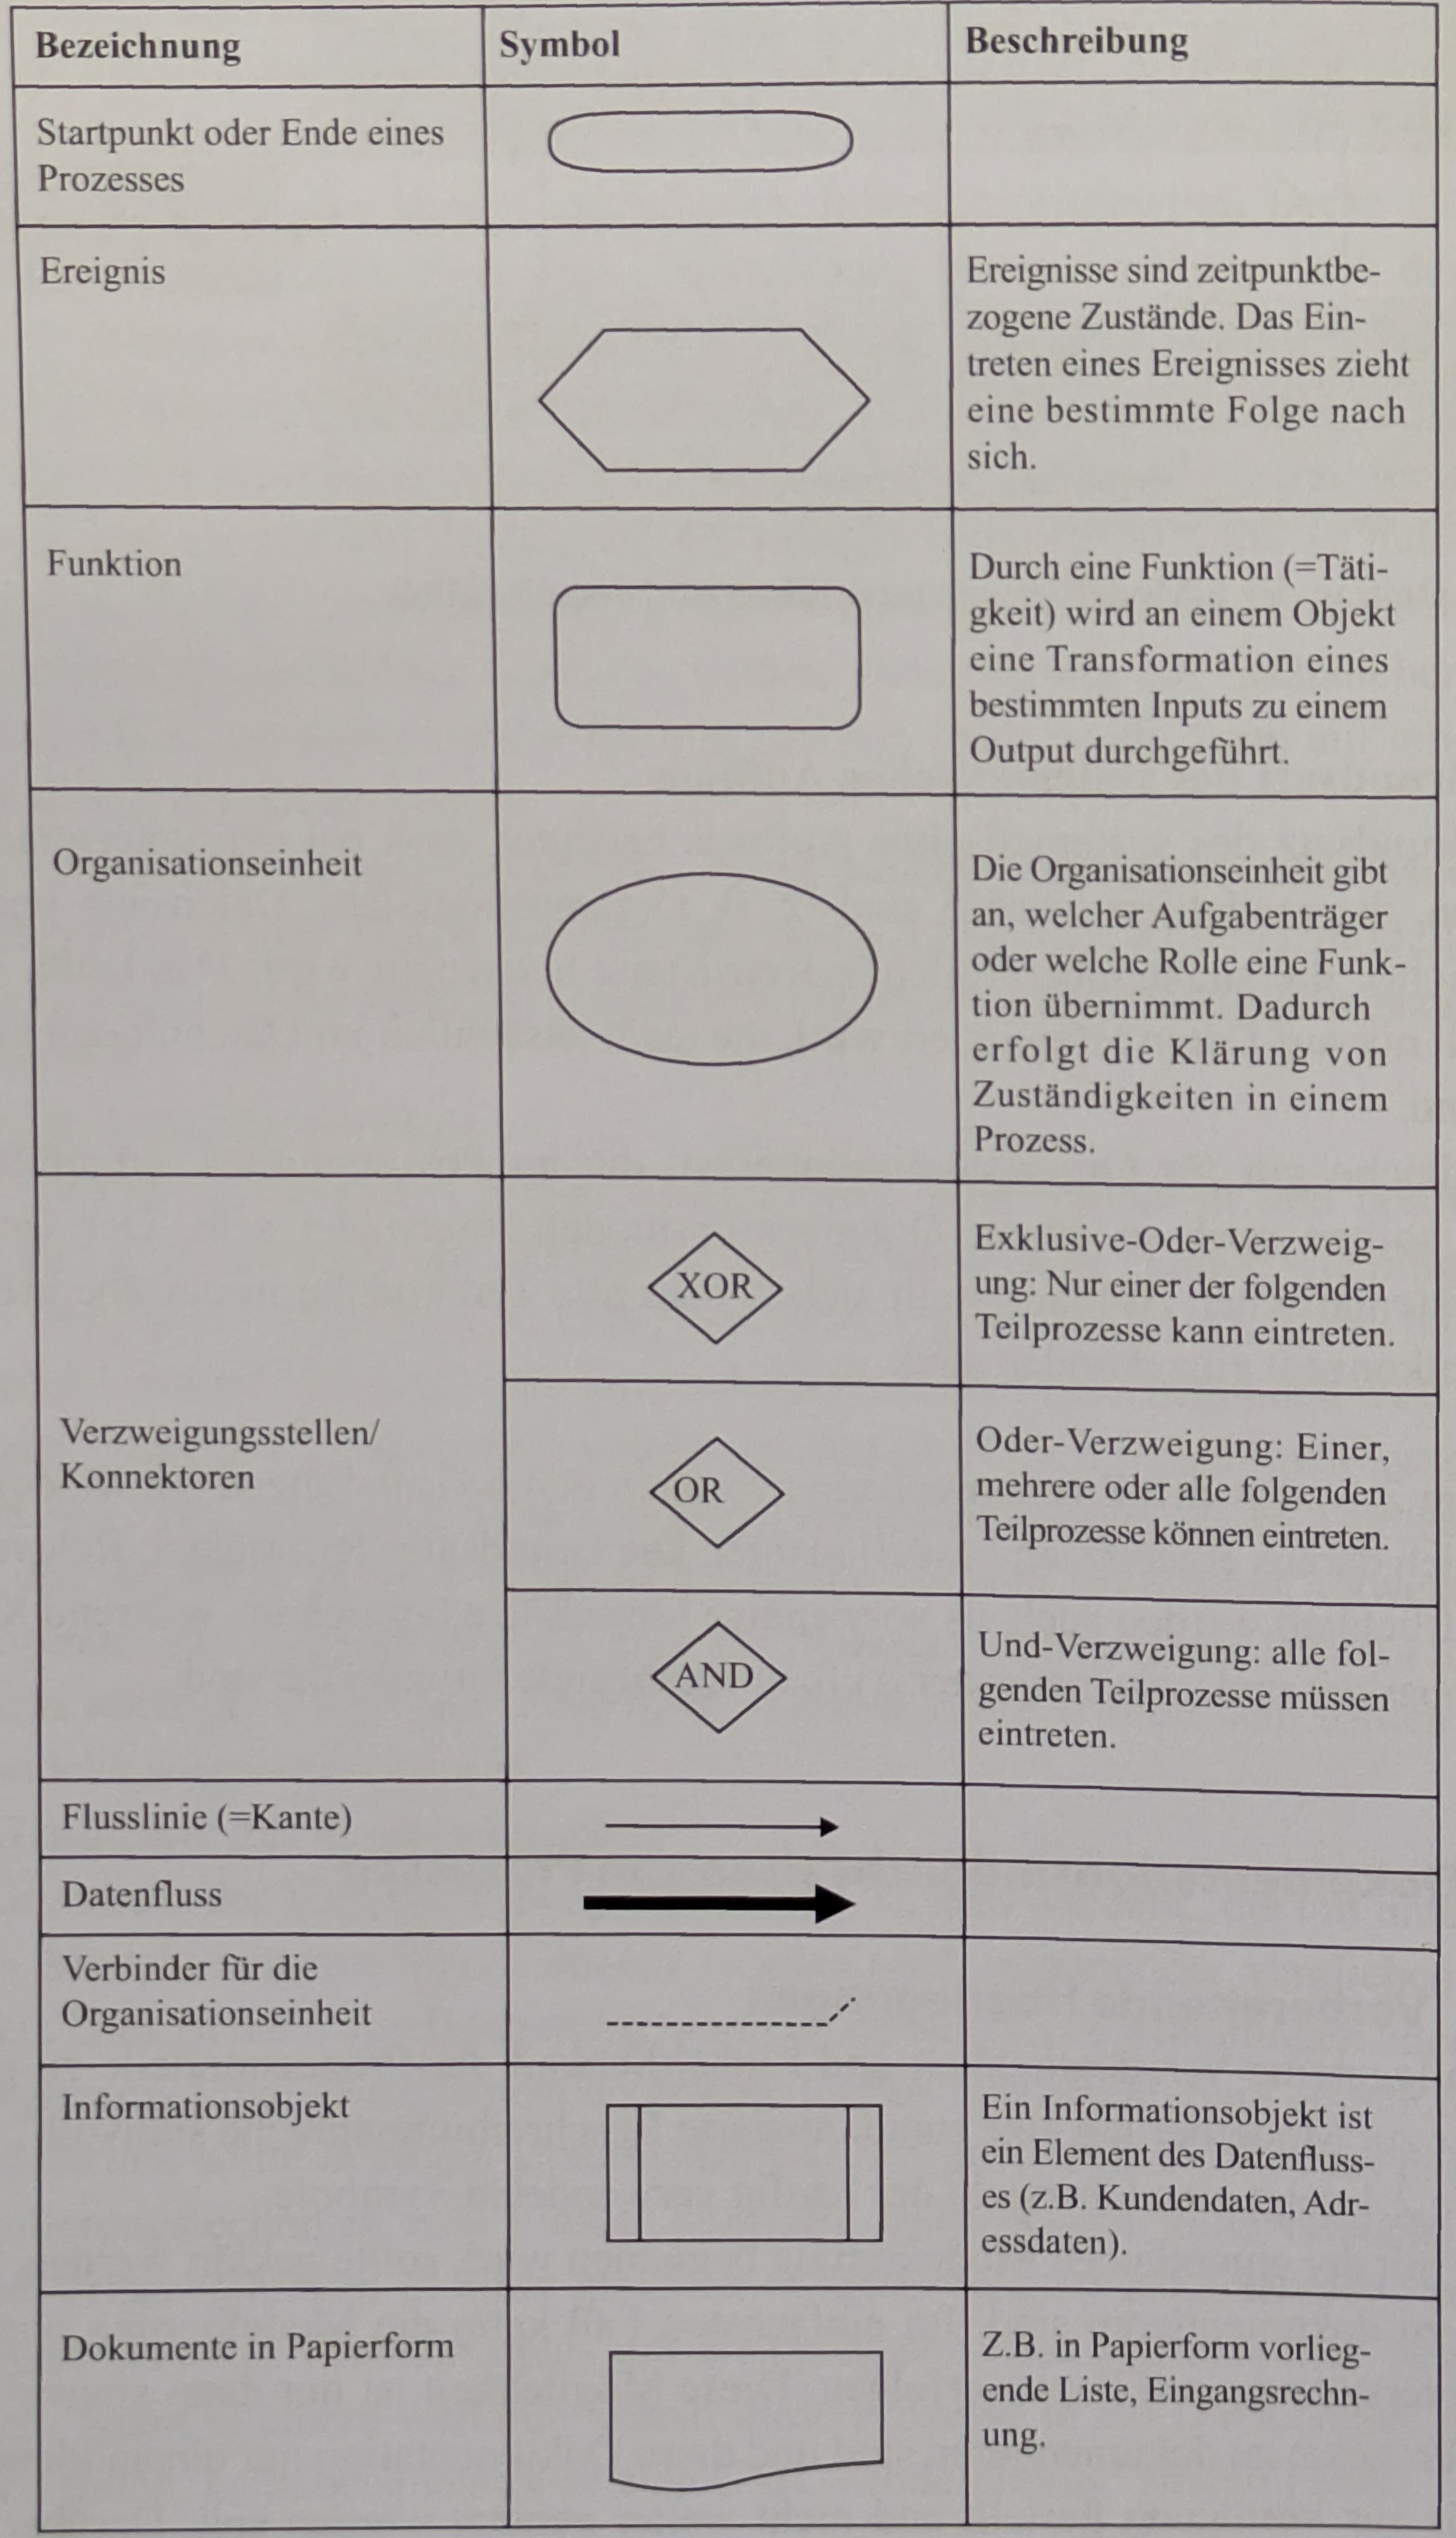
\includegraphics[width=0.8\textwidth]{BILDER-PTB3/symbole_prozessen1.jpg}
\end{center}

\newpage
\vspace*{\fill}
\begin{center}
    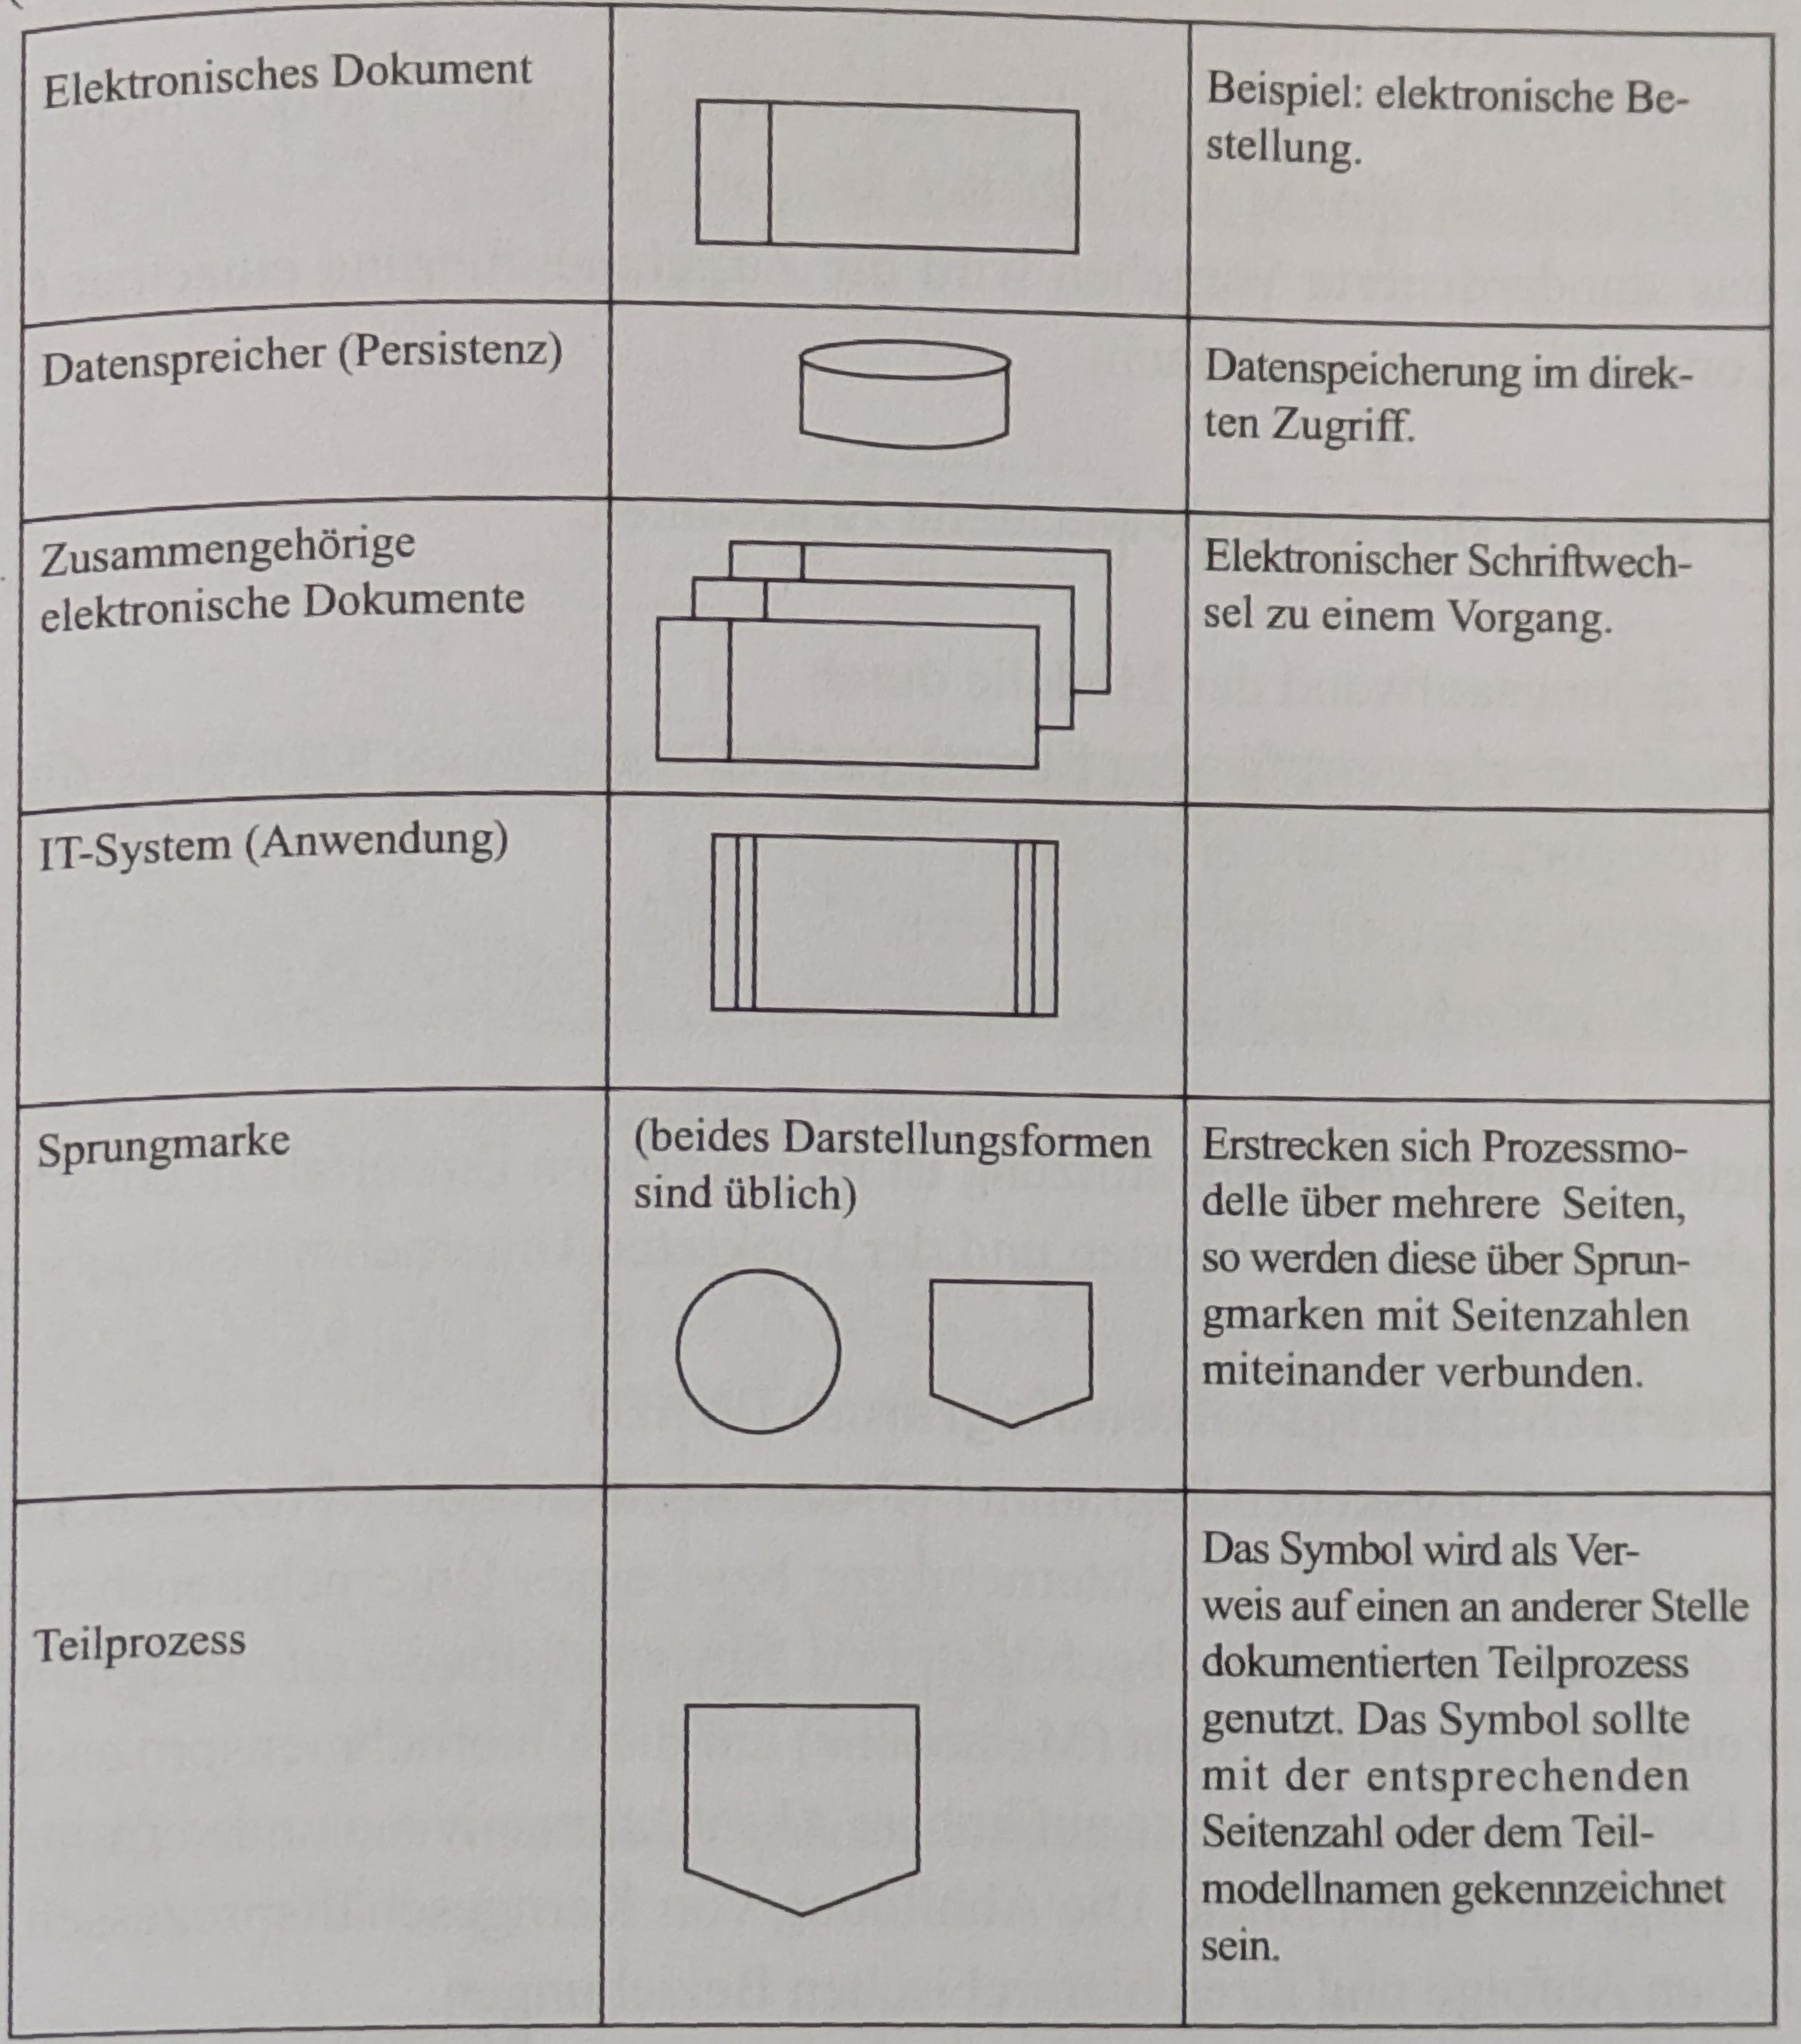
\includegraphics[width=0.85\textwidth]{BILDER-PTB3/symbole_prozessen2.jpg}
\end{center}
\vspace*{\fill}

% Anhang 2
\newpage
\phantomsection
\addcontentsline{toc}{subsection}{Anhang 2: Beteiligungsprozess bei den BWB}
\label{sec:Anhang2}
\begin{center}
    {\Large\bfseries Anhang 2: Beteiligungsprozess bei den BWB}\\[0.5cm]
    {\normalsize interne Quelle: detaillierte Beteiligungsprozess-Darstellung zur Einführung neuer Microsoft-365-Apps}\\[0.3cm]
    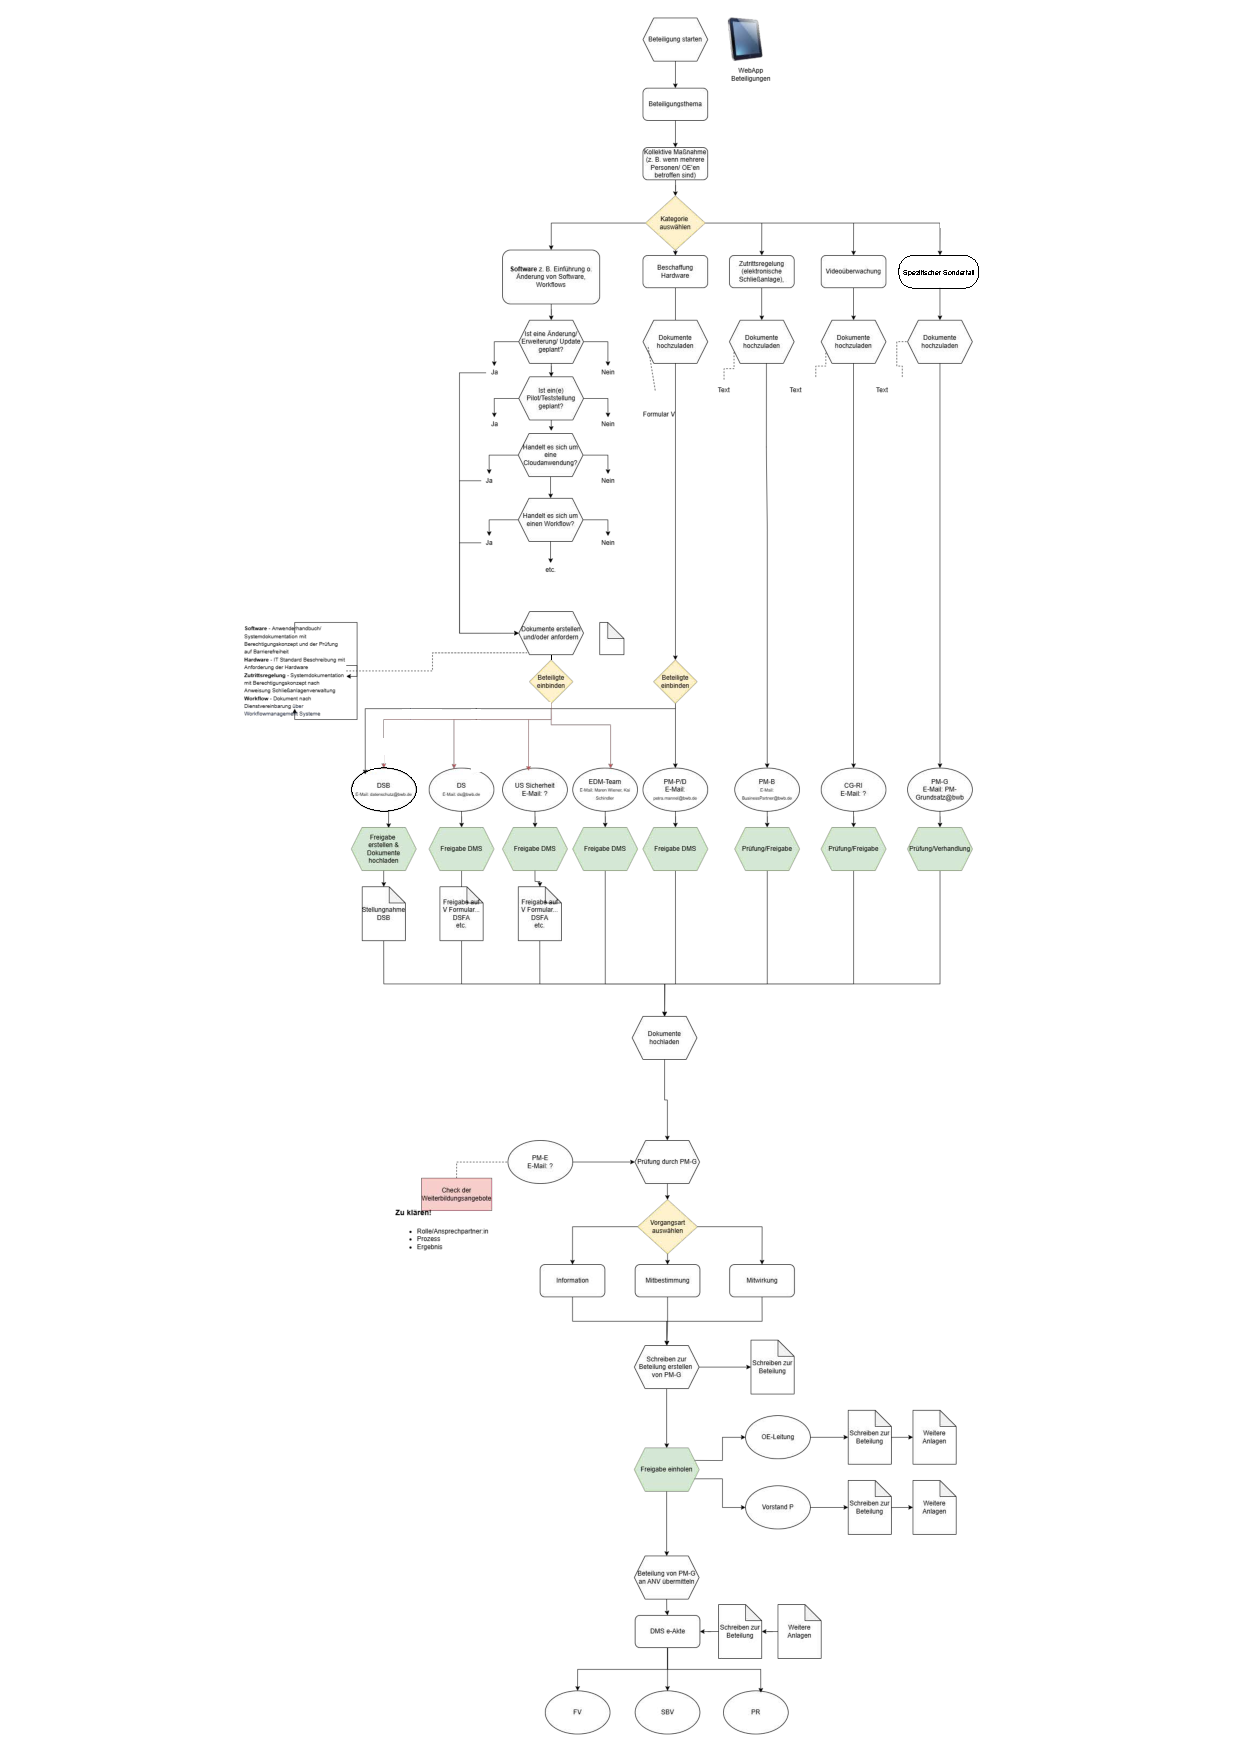
\includegraphics[width=0.97\textwidth]{BILDER-PTB3/beteiligungsprozess_software.pdf}
\end{center}

% Anhang 3
\newpage
\phantomsection
\addcontentsline{toc}{subsection}{Anhang 3: Darstellung des ADKAR-Modells}
\label{sec:Anhang3}
\vspace*{\fill}
\begin{center}
    \begin{adjustbox}{rotate=90, center, valign=b}
        \begin{minipage}{0.95\textheight}
            \centering
            {\Large\bfseries Anhang 3: Darstellung des ADKAR-Modells}\\[1em]
             {\normalsize Quelle: Eigene Darstellung in Anlehnung an das ADKAR-Modell}\\[1.0cm]
            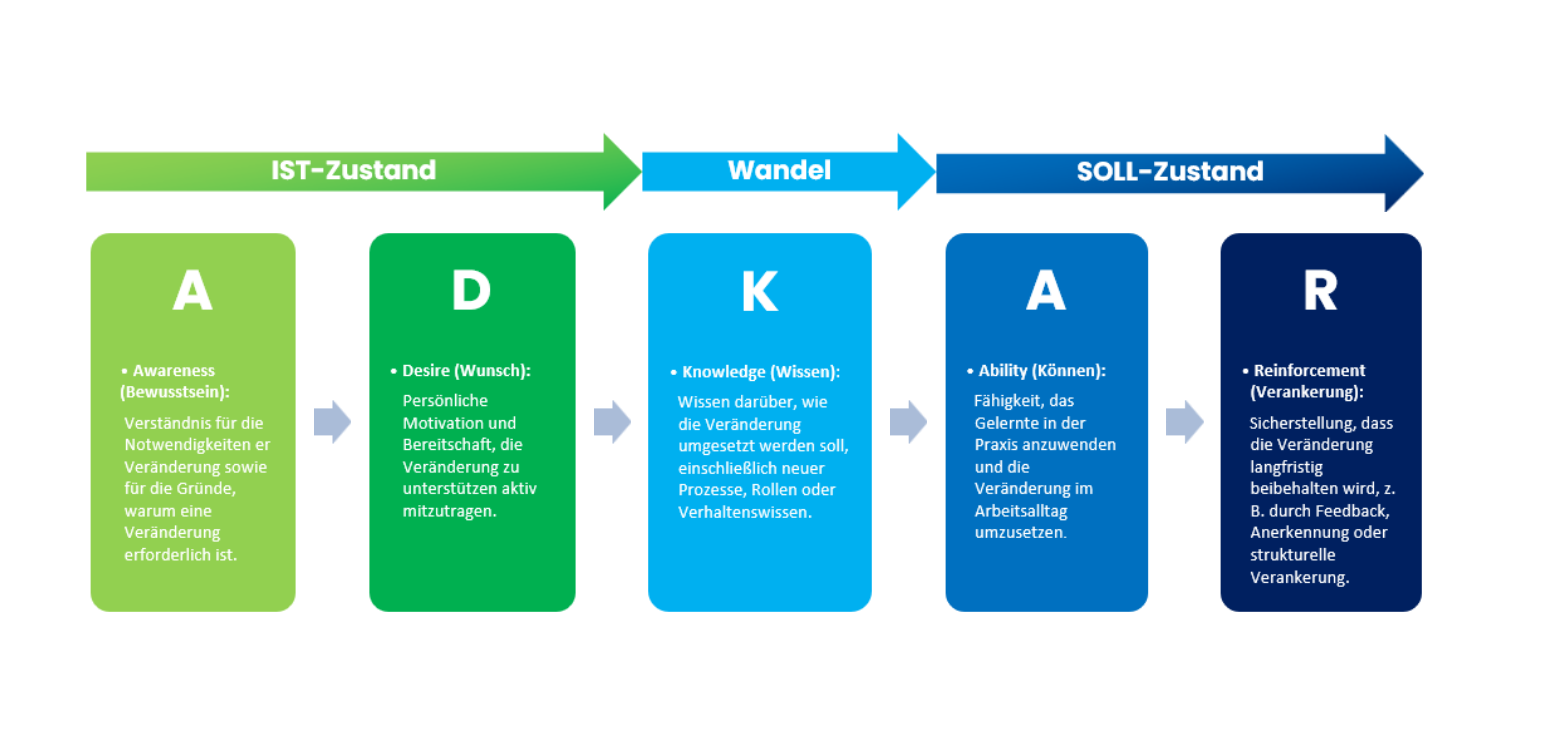
\includegraphics[width=\textheight]{BILDER-PTB3/adkar_anhang3.png}
        \end{minipage}
    \end{adjustbox}
\end{center} 

% Anhang 4
\newpage
\phantomsection
\addcontentsline{toc}{subsection}{Anhang 4: Schulungs- und Kommunikationsprozess bei den BWB}
\label{sec:Anhang4}
\begin{center}
    {\large\bfseries Anhang 4: Schulungs- und Kommunikationsprozess bei den BWB}\\[0.2cm]
    {\normalsize Quelle: Eigene Zusammenfassung des Einführungsprozesses neuer Microsoft-365-Apps mit Schulungs- und Kommunikationsprozess} \\[0.2cm]
    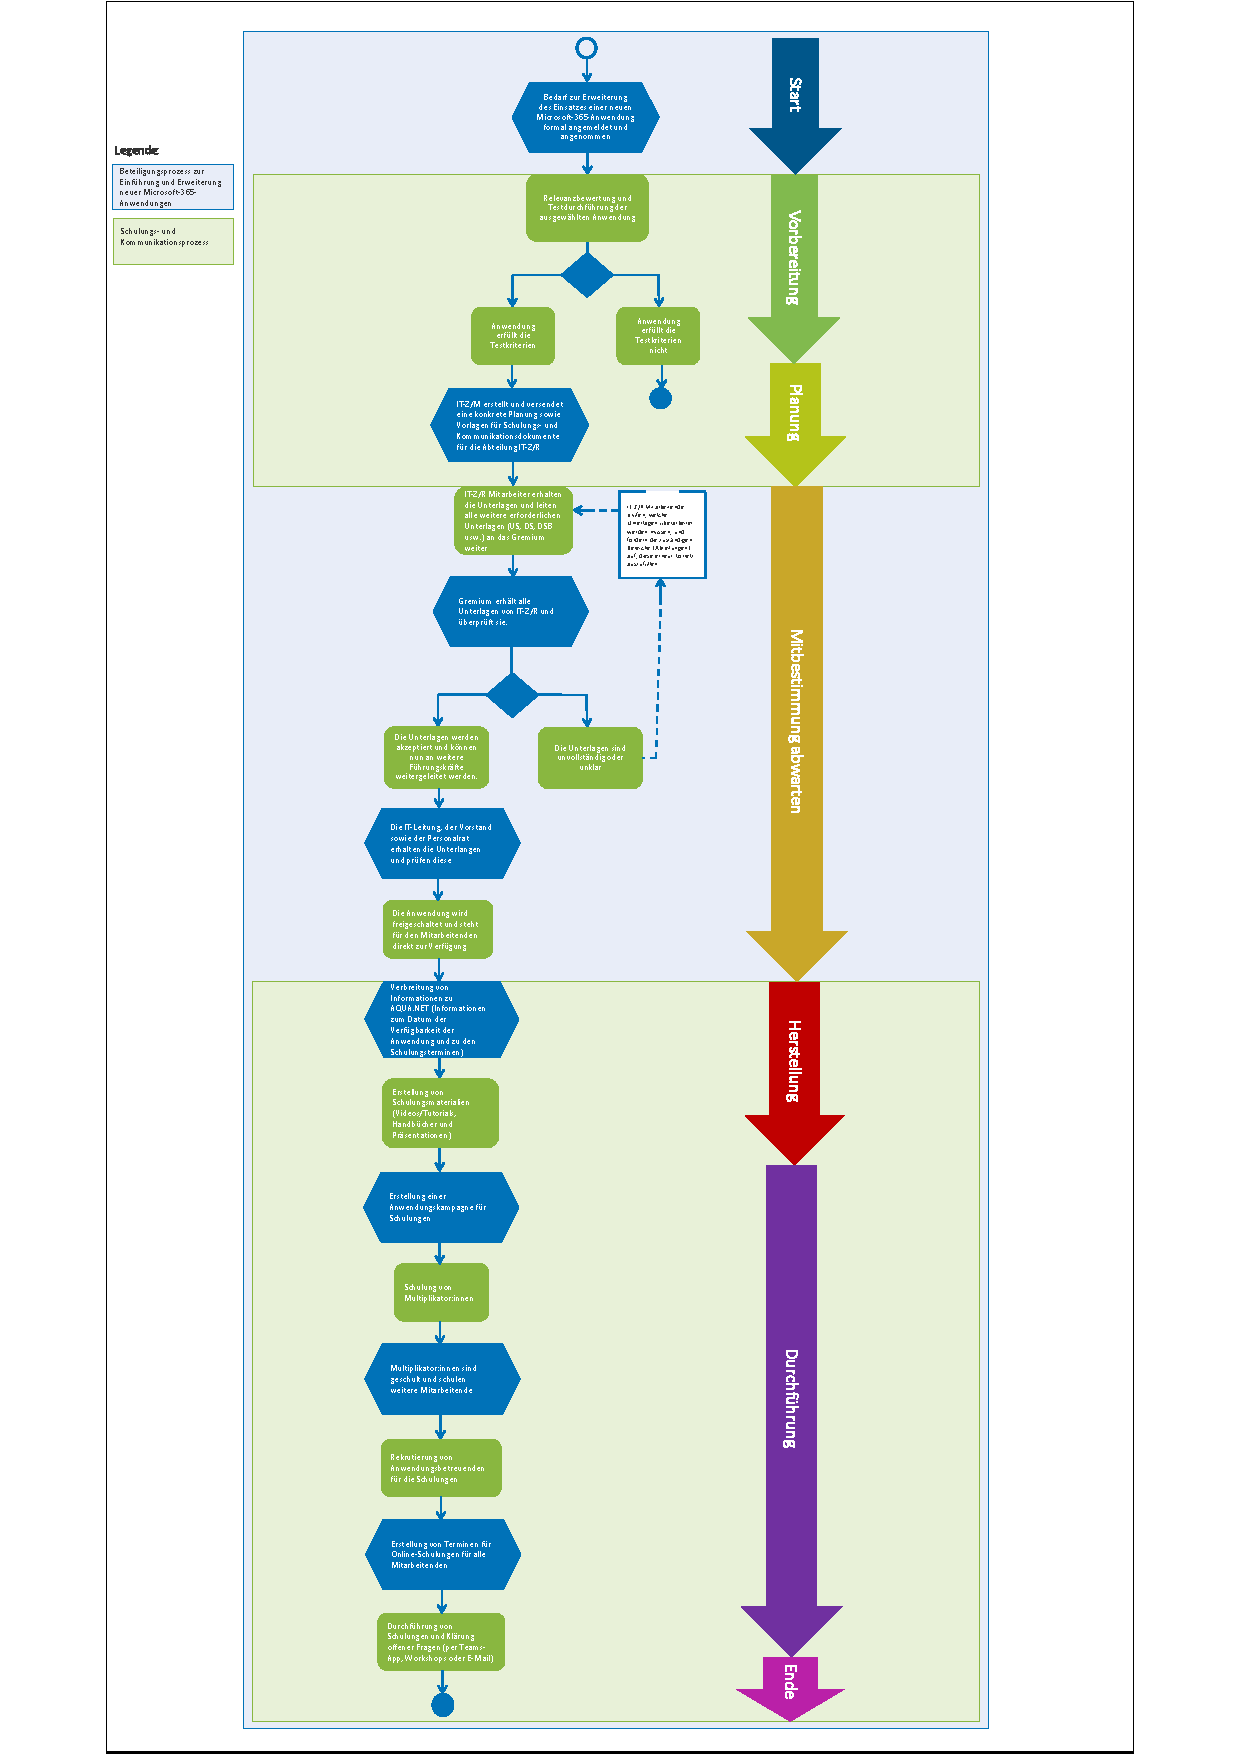
\includegraphics[width=0.81\textwidth]{BILDER-PTB3/beteiligungsprozess_schulungs_komunikationsprozess.pdf}
\end{center}

% Anhang 5
\newpage
\phantomsection
\addcontentsline{toc}{subsection}{Anhang 5: Interviewprotokoll (Diana Jimenez)}
\label{sec:Anhang5}

{\Large\bfseries Anhang 5: Interviewprotokoll}\\[1em]
\textbf{Interviewer:} Nicole Camille Baião \\
\textbf{Befragte:} Diana Ireri Jimenez Ireta (Leiterin und Beraterin von Microsoft-365-Apps, IT-Z/M) \\
\textbf{Datum:} 03. Februar 2026 \\
\textbf{Ort:} Berliner Wasserbetriebe, Neue Jüdenstraße 2, 10179 Berlin \\

\textbf{Frage 1: Welche Rolle hatten Sie bei der Einführung von Microsoft Planner und To Do?}

Diana: Im Jahr 2022 habe ich in unserer IT-Abteilung (IT-Z/M) die Verantwortung dafür übernommen, die Microsoft-365-Anwendungen im Unternehmen einzuführen und Schulungen sowie Betreuung dafür zu koordinieren. Obwohl die BWB das Microsoft-365-Paket bereits seit einiger Zeit besitzt, wurden die einzelnen Anwendungen erst im Rahmen des Beteiligungsprozesses nach und nach freigeschaltet. Die Einführung von Planner und To Do stellt daher eine neue Anwendungseinführung bzw. eine Erweiterung der bestehenden Systemlandschaft dar. Zunächst habe ich eng mit einem Kollegen zusammengearbeitet, der als Projektleiter im Modern-Workplace-Projekt tätig war. Schritt für Schritt habe ich dann immer mehr Aufgaben übernommen. Von Anfang an war ich in die Planung eingebunden. Meine Hauptaufgabe war es vor allem, die praktische Umsetzung der Einführung zu übernehmen: zu organisieren, \textit{wie wir die neuen Apps den BWB-Mitarbeiterinnen und -Mitarbeitern bereitstellen und vermitteln}.

Der gesamte Schulungs- und Kommunikationsprozess hängt eng mit dem Beteiligungsprozess zusammen. Sobald ein Bedarf für eine neue Anwendung festgestellt wird, bin ich direkt beteiligt. Ich führe dann mit meinem Team Tests durch und überprüfe, ob das Tool relevant ist und sich eine Einführung lohnt. Wenn das passt, beginne ich, konkrete Schulungsmaterialien zu erstellen, stimme mich mit IT-Z/R ab und versende die Unterlagen zur Genehmigung. Danach muss ich abwarten, bis die Mitbestimmung durchlaufen ist und wir die offizielle Freigabe erhalten. Ohne die Mitbestimmung darf ich nicht mit der Erstellung von Schulungsmaterialien und der Kommunikation mit den Mitarbeitenden beginnen. Die Schulungsmaterialien umfassen vor allem Benutzerhandbücher, Präsentationen und Tutorial-Videos. 

Sobald wir die Freigabe haben, geht es weiter mit dem Schulungs- und Kommunikationsprozess: Wir schulen die Multiplikatoren also ausgewählte Mitarbeiterinnen und Mitarbeiter, die dann weitere Kolleginnen und Kollegen in ihren Abteilungen schulen. Wenn alle Schulungsmaterialien fertig sind, organisiere ich Werbung für die neuen Online-Schulungen und halte das Ganze in Bewegung. Es ist also kein linearer Prozess, eher ein permanentes Mitdenken und Nachjustieren. Eine externe Beraterin – ein Dienstleister, den die BWB beauftragt hat – hat uns geholfen, den Schulungs- und Kommunikationsprozess mit dem Beteiligungsprozess zu verbinden. Sie hat uns anfangs beraten, und ich habe die Zusammenarbeit koordiniert. Gemeinsam mit dieser Expertin haben wir überlegt, wie wir Schulungsunterlagen und Erklärvideos am besten erstellen. Auf dieser Grundlage habe ich dann die Schulungsmaterialien ausgearbeitet und die Einführung der Tools intern begleitet.

\textbf{Frage 2: Welche Schulungsmaßnahmen wurden zur Einführung angeboten?}

Diana: Wir haben mehrere Schulungsformate parallel eingesetzt. Zum einen gab es Live-Schulungen für Mitarbeitende – teils in Form von Workshops oder Online-Sessions –, in denen wir die Funktionen von Planner und To Do vorgestellt haben. Anfangs haben wir sogar mit sogenannten Multiplikatoren gearbeitet, also einigen ausgewählten Mitarbeitenden, die wir intensiver geschult haben und die dann in ihren Teams als Ansprechpartner dienen konnten. Zum anderen haben wir den Kolleginnen und Kollegen viele Selbstlern-Materialien an die Hand gegeben. Wie erwähnt, haben wir schriftliche Anleitungen (Handbücher) sowie Präsentationsfolien erstellt, damit jeder die Schritte nachvollziehen kann. Außerdem standen kurze Erklärvideos zur Verfügung, die wir intern bereitgestellt haben. Diese Mischung aus direkten Schulungen und unterstützenden Unterlagen sollte sicherstellen, dass unterschiedliche Lernbedürfnisse abgedeckt werden. Insgesamt haben wir versucht, die Einführung möglichst durchdacht zu begleiten, indem wir sowohl persönliche Erklärungen als auch Unterlagen zum Nachlesen und -schauen angeboten haben.

\textbf{Frage 3: Wie wurden die Mitarbeitenden über Planner und To Do informiert?}

Diana: Die interne Kommunikation über die neuen Tools lief hauptsächlich über unser Intranetportal AQUA.net. Dort haben wir mehrfach Artikel veröffentlicht, um die Belegschaft über Planner und To Do zu informieren – z.B. Ankündigungen zur Einführung und Tipps zur Nutzung. AQUA.net ist der zentrale digitale Infokanal bei uns, auf dem alle Neuigkeiten geteilt werden. Im Laufe des Einführungsprozesses haben wir also zu mehreren Zeitpunkten Beiträge eingestellt, um die Mitarbeitenden auf dem Laufenden zu halten. Zusätzlich haben wir natürlich in Meetings und via E-Mail auf Schulungsangebote hingewiesen, aber der Hauptkanal war das Intranet. Wichtig war uns, immer wie der an die neuen Möglichkeiten zu erinnern und Hilfestellungen anzubieten, damit Planner und To Do wahrgenommen werden.

\textbf{Frage 4: Wie bekannt sind die neuen Tools unter den Mitarbeitenden?}

Diana: Trotz unserer Informationskampagne muss man sagen, dass nicht alle Mitarbeitenden die neuen Anwendungen kennen. Ich schätze, dass etwa 60–70\,\% der Belegschaft mitbekommen haben, dass es Planner und To Do gibt. Viele wissen aber nicht genau, wofür diese Tools eigentlich gedacht sind oder welchen Mehrwert sie bieten. Ein Problem ist sicherlich, dass zwar alle offiziellen Mitteilungen auf AQUA.net stehen, aber nicht jeder Mitarbeitende liest regelmäßig das Intranet. Einige Kollegen – speziell draußen im technischen Bereich – fühlen sich von der ganzen digitalen Informationsflut eher überfordert und meiden solche Plattformen teilweise. Für diese Gruppen gingen die Informationen möglicherweise unter. Hinzu kommt, dass Planner und To Do freiwillige Tools sind – niemand wird von oben dazu verpflichtet, sie zu nutzen. Entsprechend haben manche von vornherein nicht genauer hingeschaut. Insgesamt würde ich sagen, rund zwei Drittel haben zumindest von den Tools gehört. Aktiv nutzen tun sie aber deutlich weniger Mitarbeiter. Mein Gefühl ist, dass momentan vielleicht maximal zehn Prozent der Beschäftigten Planner oder To Do tatsächlich regelmäßig einsetzen. Die Einführung liegt ja auch erst wenige Monate zurück, da ist viel noch in der Ausprobierphase. Nach meiner Erfahrung dauert es in unserem Unternehmen um die fünf Jahre, bis sich ein neues Tool wirklich breit etabliert hat und selbstverständlich genutzt wird.

\textbf{Frage 5: Warum erkennen manche Mitarbeitende den Mehrwert von Planner und To Do nicht?}

Diana: Viele Kollegen stehen neuen Tools anfangs skeptisch gegenüber. Wenn etwas Neues kommt, reagieren manche beinahe ängstlich, als wäre es eine völlig fremde Welt. Ich erlebe oft, dass Veränderungen Überforderung auslösen – die Leute fühlen sich von neuen Anwendungen eher erschlagen. Aus Gesprächen mit Kolleginnen und Kollegen habe ich den Eindruck, dass sich viele mehr Unterstützung an der Hand wünschen würden, also eine ganz enge Anleitung nach dem Motto: „Klick zuerst hier, dann dort…“ Diese Führung haben wir auch versucht zu bieten, etwa durch Schritt-für-Schritt-Demos in den Schulungen. Dennoch beobachtet man eine große Bandbreite: Während ein Teil der Mitarbeitenden sehr technikaffin ist und neue Tools wie Planner sofort intuitiv ausprobiert, tun sich andere viel schwerer damit. Es gibt quasi zwei Lager – oft auch entlang der Generationen.

Jüngere Kolleg*innen haben meist Spaß daran, neue digitale Hilfsmittel auszuprobieren, und bringen sich vieles selbst bei. Ältere Mitarbeitende dagegen empfinden solche Tools häufiger als kompliziert und lästig. Ihre Hemmschwelle ist höher, und sie bleiben lieber bei den gewohnten Arbeitsweisen. In der Tat hat es bei uns z. B. Jahre gedauert, bis Confluence (das interne Wiki) von allen akzeptiert und genutzt wurde – anfangs hieß es auch, das sei unübersichtlich und so weiter. Erst nach fünf Jahren war das Tool wirklich integriert im Arbeitsalltag. Jetzt kommen wir mit noch neueren Anwendungen wie Planner, die ähnliches können, und da fragen erfahrene Kolleg*innen natürlich: „Wozu das Ganze? Warum sollen wir schon wieder wechseln?“ Dieses Gefühl, bereits Bewährtes zu haben, lässt manche den Nutzen eines weiteren Tools infrage stellen. Wie gesagt, einige informieren sich auch schlicht nicht, weil sie gar kein Interesse daran haben. Und diejenigen, die Bescheid wissen, nutzen Planner und To Do teilweise trotzdem nicht, weil sie es nicht möchten – es ist ja, wie erwähnt, kein Zwang. Diese Vorbehalte und die Zurückhaltung gehören zu den größten Hürden bei der Verbreitung der neuen Tools.

\textbf{Frage 6: Was waren die größten Herausforderungen bei den Schulungen?}

Diana: In den Schulungen selbst war die Teilnehmende auf ganz unterschiedlichen Kenntnisstufen eine echte Herausforderung. Häufig saßen in einer Session Kolleg*innen mit sehr unterschiedlichen Vorkenntnissen zusammen. Da den richtigen Tempo-Mix zu finden, war schwierig: Entweder war ich für die einen zu langsam, oder für die anderen zu schnell. Zum Beispiel hatten einige das Prinzip sofort intuitiv verstanden, während andere bei jeder neuen Funktion erst einmal ins Stocken gerieten. Aus dieser Erfahrung habe ich gelernt und meine Herangehensweise angepasst: Künftig würde ich die Trainingsgruppen nach Wissensstand trennen und vorab abfragen, wer schon Vorerfahrung mitbringt. So kann man Einsteiger und Fortgeschrittene getrennt schulen. Außerdem ist es besser, weniger Inhalte pro Termin zu vermitteln und dafür die Anzahl der Schulungstermine zu erhöhen. Wir haben am Anfang vielleicht zu viel auf einmal zeigen wollen – alle Funktionen in einer Sitzung – und damit einige überfordert. Besser ist es, kleinere Lerneinheiten zu machen. So bleibt jeder dran, ohne dass die einen sich langweilen und die anderen überfordert sind. Diese Aufteilung nach Niveau und Häppchenbildung des Stoffs hat sich für mich als wichtige Lektion aus den ersten Schulungen ergeben.

\textbf{Frage 7: Wie können die Schulungs- und Kommunikationsprozesse verbessert werden?}

Diana: Aus heutiger Sicht würde ich vorschlagen, unsere Schulungs- und Kommunikationsstrategie noch gezielter auf die verschiedenen Zielgruppen zuzuschneiden. Zum einen könnten wir bei den Schulungen stärker nach Altersgruppen oder Vorkenntnissen differenzieren. Beispielsweise bräuchten ältere Kolleg*innen oder generell diejenigen mit wenig IT-Erfahrung vielleicht noch ausführlichere Erläuterungen – für sie wären zusätzliche, detaillierte Tutorials oder Videos hilfreich. Jüngeren und versierteren Nutzergruppen reichen oft schon kurze Übersichten oder Workshops, um den Einstieg zu finden. Hier könnten wir also vom Umfang her variieren, damit jeder weder unterfordert noch überfordert wird. Zum anderen sollten wir bei der internen Kommunikation neue Wege gehen. 

Wie besprochen, ist AQUA.net als einziges Medium nicht genug, weil es gewisse Mitarbeiterkreise nicht erreicht. Man könnte überlegen, weitere Kanäle einzusetzen, um über Neuerungen wie Planner und To Do zu informieren. Zum Beispiel wurde intern die Idee diskutiert, eine Art unternehmensweiten Chat oder Social Feed einzurichten, wo alle Beschäftigten Neuigkeiten mitbekommen. So etwas wie ein zentraler Teams-Kanal für die ganze BWB existiert zwar, aber er wird nicht von allen genutzt– vielleicht braucht es ein noch niedrigschwelligeres Kommunikationstool, das wirklich jeden erreicht. Kurz gesagt: Wir sollten parallel zum Intranet andere Kommunikationswege ausprobieren, um auch die Mitarbeitenden abzuholen, die bisher kaum Informationen mitbekommen. Wenn wir Schulungsangebote zielgruppengerechter gestalten und die Informationsverbreitung breiter aufstellen, könnten künftige Einführungsprozesse vermutlich deutlich effizienter und erfolgreicher verlaufen.

% Anhang 6
\newpage
\phantomsection
\addcontentsline{toc}{subsection}{Anhang 6: Interviewprotokoll (Nicolas Zoll)}
\label{sec:Anhang6}

{\Large\bfseries Anhang 6: Interviewprotokoll}\\[1em]
\textbf{Interviewer:} Nicole Camille Baião \\
\textbf{Befragte:} Nicolas Zoll (Risikomanager, IT-Z/R) \\
\textbf{Datum:} 05. Februar 2026 \\
\textbf{Ort:} Berliner Wasserbetriebe, Neue Jüdenstraße 2, 10179 Berlin \\

\textbf{Frage 1: Welche Rolle haben Sie im Beteiligungsprozess zur Einführung neuer Softwareprodukte?}

Nicolas Zoll: Meine Aufgabe ist es, den Beteiligungsprozess bei neuen Software-Einführungen zu koordinieren. Ich bin Risikomanager (und auch für Qualitätsmanagement zuständig) und arbeite im Abteilung IT-Z/R (IT-Zentrale Aufgaben – Risk Complance and Security). Unsere Bereichsleitung hat mich und eine Kollegin (Leiterin von IT-Z/R) benannt, um alle Beteiligungsvorgänge zu betreuen. Wir selbst erstellen die erforderlichen Dokumente nicht – das machen die jeweiligen Projekt- oder Fachverantwortlichen des neuen Tools. Stattdessen stellen wir sicher, dass alle Unterlagen vollständig vorliegen, und beraten die Kollegen, was genau eingereicht werden muss. Kurz gesagt: Wir begleiten und steuern den Prozess beratend im Hintergrund, damit am Ende sämtliche nötigen Freigaben und Dokumente für das Beteiligungsverfahren vorhanden sind.

\textbf{Frage 2: Wie läuft der Prozess ab, wenn eine neue Software eingeführt werden soll, und wer ist wann beteiligt?}

Nicolas Zoll: Zunächst muss der Bedarf für das neue Softwareprodukt formal angemeldet werden. Die zuständige Projektleitung (bzw. Fachabteilung) bereitet einen Einführungsantrag vor – in Form eines \textit{„Whitepapers zur Beteiligung“}. In dieser standardisierten Vorlage werden die Grunddaten des Vorhabens festgehalten (Ansprechpartner, betroffene Bereiche, geplantes Einführungsdatum etc.). Parallel dazu erstellt das Projekt eine kurze Beschreibung der Software und ihrer Funktionen sowie ein Berechtigungskonzept. Bereits in dieser frühen Phase werden wichtige Stellen vorab eingebunden: So findet eine Abstimmung mit dem IT-internen Datenschutz-Team, dem sogenannten EDM-Team als technische Experten der Arbeitnehmervertretung) statt, um das Vorhaben technisch mit der Arbeitnehmerseite vorzuklären. Ebenso muss der Datenschutzbeauftragte (DSB) frühzeitig eingebunden werden und eine schriftliche Stellungnahme abgeben, dass aus Datenschutz-Sicht nichts gegen die Einführung spricht. Handelt es sich um eine Cloud-Anwendung, wird zusätzlich die Datenschutz-Fachabteilung (DS). Außerdem schaltet die IT die Unternehmenssicherheit (Abteilung US) ein: Gemeinsam wird eine Schutzbedarfsfeststellung durchgeführt, um das Sicherheitsniveau des neuen Tools einzuschätzen (Quick-Scan mit entsprechenden Fragen zur Anwendung). Bereits hier werden also Datenschutz und IT-Security eng einbezogen.

Sobald alle Unterlagen ausgearbeitet sind und die nötigen Vorab-Freigaben eingeholt, wird das Gesamtpaket an Dokumenten zunächst im Personalmanagement-Abteilung also das Gremium (PM-G) überprüft, ob die Dokumentenanforderungen erfüllt sind und werden danach abgestimmt. Als nächstes wird der Vorstand gemeinsam mit dem IT-Leiter darauf, jede Software-Einführung vor der offiziellen Einreichung einmal zu prüfen. Wenn alles korrekt ist, wird den Vorgang in das eigentliche Beteiligungsverfahren an den Personalrat weiter. Dort wird der Vorgang behandelt – der Personalrat hat die Mitbestimmung und muss dem Einsatz der neuen Software zustimmen - wird weitergeleitet (je nach Bereich an den Personalrat der Hauptverwaltung, Wasser oder Abwasser). Durch diese extra Schleife stellen wir sicher, dass die Leitung früh informiert ist und der Personalrat später nicht mit unvollständigen Informationen konfrontiert wird.  Liegt schließlich die Zustimmung des Personalrats vor, darf die Software produktiv ausgerollt werden. Erst nach dieser formalen Freigabe ist die Einführung offiziell abgeschlossen und das Tool kann unternehmensweit genutzt werden.

\textbf{Frage 3: Welche Dokumente und Materialien müssen für das Beteiligungsverfahren vorbereitet werden?}

Nicolas Zoll: Für die Einführung eines neuen Tools ist eine ganze Reihe von Unterlagen erforderlich. Insbesondere müssen wir folgende Dokumente bündeln:
\begin{itemize}
    \setlength\itemsep{0.4\baselineskip}
    \setlength\parskip{0pt}
    \setlength\parsep{0pt}
    \item \normalsize ein Whitepaper zur Beteiligung – die offizielle Vorlage mit den Basisinformationen zum Vorhaben (Art der Software, Bedarf, Ansprechpartner, Zeitplan usw.),
    \item \normalsize eine fachliche Beschreibung der Software (inklusive der vorgesehenen Funktionalitäten und eines Berechtigungskonzepts zur Rechtevergabe),
    \item \normalsize eine Schutzbedarfsfeststellung (IT-Sicherheitsbewertung) in Zusammenarbeit mit der Unternehmenssicherheit – oft in Form eines Quick-Scans mit definierter Checkliste,
    \item \normalsize sämtliche Datenschutz-Dokumente: insbesondere das Verzeichnis von Verarbeitungstätigkeiten (VVT) für das neue Tool, ein entsprechendes Löschkonzept sowie eine initiale Datenschutz-Risikoanalyse; falls diese ergibt, dass ein hohes Risiko vorliegt, kommt noch eine ausführliche Datenschutz-Folgenabschätzung hinzu,
    \item \normalsize die schriftlichen Freigaben/Stellungnahmen der Datenschutzinstanzen – also eine Einwilligung des Datenschutzbeauftragten (DSB) und ggf. zusätzlich eine Stellungnahme der Datenschutz-Abteilung (DS), falls diese beteiligt werden muss (z. B. bei Cloud-Themen),
    \item \normalsize ein Schulungskonzept und Anwender-Unterlagen für die Beschäftigten – beispielsweise Benutzerhandbücher, Präsentationen oder Lernvideos. Diese Materialien dienen dazu, die Mitarbeiter auf das neue Werkzeug vorzubereiten. Die Arbeitnehmervertretung fragt im Beteiligungsverfahren gezielt nach solchen Schulungsmaßnahmen, um sicherzustellen, dass alle Anwender mit der eingeführten Software umgehen können.
\end{itemize}
Alle diese Unterlagen müssen von den Projektverantwortlichen vorbereitet und im Zuge des Antrags eingereicht werden. Unsere Aufgabe in IT-Z/R ist es, darauf zu achten, dass diese Dokumente vollständig vorliegen und inhaltlich mit den zuständigen Stellen (DSB, DS, US etc.) abgestimmt sind, bevor wir den Antrag weiterleiten.

\textbf{Frage 4: Welche typischen Probleme treten im aktuellen Beteiligungsprozess auf?}

Nicolas Zoll: Aus meiner Sicht ist der Prozess momentan sehr aufwendig und zeitintensiv. Ein Hauptproblem ist der hohe Abstimmungsaufwand: Es sind zu viele Parteien involviert – vom Datenschutzbeauftragten über die Datenschutz-Abteilung und die Unternehmenssicherheit bis hin zu mehreren Gremien der Personalvertretung. Jede dieser Stellen muss nacheinander eingebunden werden, was zu erheblichen Verzögerungen führt. Je mehr Leute mitreden, desto länger dauert am Ende die Einführung. Hinzu kommt ein enormer Dokumentationsaufwand: Für jedes Vorhaben müssen unzählige Formulare, Konzepte und Stellungnahmen erstellt werden. Viele dieser Unterlagen überschneiden sich inhaltlich, was zu Medienbrüchen und Doppelarbeit führt – man pflegt ähnliche Informationen in verschiedenen Dokumenten und Systemen parallel. Das macht den Ablauf in der Praxis sehr mühsam und fehleranfällig.\\\\

\textbf{Frage 5: Wie könnte der Beteiligungsprozess verbessert oder beschleunigt werden?}

Nicolas Zoll: Ich sehe durchaus Potenzial, den Prozess schlanker und effizienter zu gestalten. Ein wichtiger Schritt, der bereits angegangen wird, ist die Digitalisierung des Verfahrens: Statt zig Word-Dokumenten und Excel-Listen alles manuell auszufüllen, sollte ein einheitlicher Workflow im System den Prozess abbilden. Wenn alle Informationen in einer zentralen Plattform erfasst und automatisch an die zuständigen Stellen weitergeleitet werden, reduzieren wir die Medienbrüche und sparen viel Zeit. Zum Glück wird so ein Workflow-System jetzt endlich eingeführt – darauf setze ich große Hoffnungen. Zudem würde ich die Anzahl der Beteiligten Instanzen reduzieren, um Doppelarbeit zu vermeiden. Beispielsweise könnte man die Datenschutz-Prüfung auf eine Instanz konzentrieren. Es würde reichen, wenn der Datenschutzbeauftragte das Vorhaben bewertet und freigibt – die zusätzliche Prüfung durch die separate Datenschutz-Abteilung könnte entfallen, denn zwei parallele Datenschutzbewertungen sind aus meiner Sicht überflüssig (zumal DSB und DS oft das Gleiche prüfen). Allgemein sollten nicht „zu viele Köche“ mitreden, da dies den Brei nur verdirbt – sprich: weniger involvierte Personen würden den Ablauf vereinfachen und beschleunigen.

Ein weiterer Verbesserungsansatz betrifft den Dokumentationsaufwand. Hier sollte geprüft werden, welche Unterlagen wirklich erforderlich sind. Viele Dokumente (etwa das VVT und das Löschkonzept) sind in der jetzigen Form pro Tool-Einführung nicht ideal, weil sie eigentlich pro Geschäftsprozess gedacht sind. Man könnte überlegen, statt für jedes neue Tool komplett neue umfangreiche Dokumente zu schreiben, eher mit vereinfachten Checklisten oder Referenzen auf bestehende Prozess-Dokumentationen zu arbeiten. Zusammengefasst würde ich mir einen schlankeren Prozess mit weniger Bürokratie wünschen. Weniger Beteiligte, klarere Zuständigkeiten und frühzeitige Abstimmung der wichtigen Punkte (Datenschutz, IT-Sicherheit) in einem digital unterstützten Workflow würden viel helfen. So könnten neue Microsoft-365-Tools deutlich schneller und reibungsloser eingeführt werden, ohne dass wichtige Prüfschritte ausgelassen werden – einfach mit weniger Overhead.

% === Ehrenwörtliche Erklärung ===
\newpage
\section*{Ehrenwörtliche Erklärung}
\addcontentsline{toc}{section}{Ehrenwörtliche Erklärung}

„Ich erkläre ehrenwörtlich:

\begin{itemize}
    \raggedright
    \item \normalsize dass ich meinen Praxistransferbericht ohne fremde Hilfe erstellt habe,
    \item \normalsize dass ich wörtliche Zitate aus der Literatur – etwa aus Büchern, wissenschaftlichen Artikeln oder offiziellen Quellen – entnommen und entsprechend gekennzeichnet habe,
    \item \normalsize dass ich Künstliche Intelligenz zur Formulierung einiger Sätze verwendet habe, und ebenfalls zur Korrektur der grammatikalischen Fehler beim Schreiben“
\end{itemize}
„Alle Quellen, die aus dem Internet oder aus anderen digitalen Medien stammen, die für den Praxistransferbericht verwendet wurden, sind der Arbeit beigefügt.“

„Ich bin mir bewusst, dass eine falsche Erklärung rechtliche Konsequenzen nach sich zieht“.\\

% --- Tabelle mit Unterschriften ---

\begin{tabular}{p{8cm}}
    \normalsize{Berlin, den XX. XXXX 202X} \\[0.5cm]
    
\includegraphics[width=5.5cm]{BILDER-PTB3/unterschrift_nicole.png} \\
    \normalsize{\underline{\hspace{5.5cm}}} \\
    \normalsize{(Unterschrift der Studentin)}
\end{tabular} % \underline{\hspace{6cm}} erzeugt eine Linie mit einer Länge von 6 cm


% === ENDE DOKUMENT ===
\end{document}
